\documentclass{foi}
\usepackage{lipsum}
\usepackage[utf8]{inputenc}
\usepackage{float}

\lstset{basicstyle=\ttfamily,
  showstringspaces=false,
  commentstyle=\color{red},
  keywordstyle=\color{blue},
}

\vrstaRada{\zavrsni}
\title{Izrada aplikacije za pronalazak termina sastanaka}

\author{Leo Ćavar}
\spolStudenta{\musko}
\mentor{Marko Mijač}
\spolMentora{\musko}
\godina{2024}
\mjesec{Rujan}
\date{2024}
\status{redoviti}
\indeks{0016153823}
\smjer{Informacijski i poslovni sustavi}
\titulaProfesora{Doc. Dr. sc.}

\sazetak{U ovom završnom radu obrađuje se korištenje .NET tehnologija za izradu programa za dogovaranje sastanaka. Rad pokriva kratki pregled ASP.NET Core i ASP.NET Web API tehnologija, uz objašnjenje koncepata API-ja i HTTP metoda. Poseban naglasak stavljen je na korištenje Google API-ja, uključujući Google Calendar API, te autentifikaciju i autorizaciju korisnika pomoću OAuth 2.0 protokola. Kroz rad se također prikazuju primjeri zahtjeva za dohvaćanje i upravljanje kalendarskim događajima, uz detaljnu implementaciju .NET web aplikacije koja omogućuje dogovaranje sastanaka među korisnicima.}

\kljucneRijeci{API; ASP. NET Core; .NET; C\#; ASP. NET; ; OAuth 2.0; Google Calendar; Google API;}

\begin{document}

\maketitle

\tableofcontents

\pagestyle{plain}
\chapter{Uvod}
U ovom radu usredotočit ćemo se na izradu programa za dogovaranje sastanaka putem Google API-ja, koji omogućuje jednostavnu interakciju s iznimno popularnim Google kalendarom. Google kalendar nudi niz funkcionalnosti koje olakšavaju organizaciju i planiranje događaja, cilj ovoga rada je iskoristiti te funkcionalnosti kako bismo omogućili lakše usklađivanje termina između više sudionika. Kroz implementaciju ovog programa, korisnici će moći u stvarnom vremenu pregledavati slobodne termine svih sudionika te na temelju tih podataka dogovarati sastanke na način koji svima odgovara. Program ćemo izraditi korištenjem ASP.NET Core frameworka, koji omogućuje razvoj web aplikacija. Razor stranice koristit ćemo za izradu korisničkog sučelja i upravljanje podacima, stvarajući intuitivno korisničko iskustvo. S druge strane, ASP.NET Web API služit će za primanje HTTP zahtjeva i komunikaciju s Google servisima, omogućujući manipulaciju događajima u kalendaru. Na taj način, uspostavit ćemo interakciju između korisnika i Google API-ja, automatizirajući procese koji bi se inače obavljali ručno. Poseban naglasak ovog rada bit će na integraciji Google Calendar API-ja s našom aplikacijom. Ovaj API omogućuje pristup informacijama o zauzetim i slobodnim terminima, kao i kreiranje, ažuriranje i brisanje događaja.
Kroz ovaj projekt prikazat ćemo tehničke aspekte integracije s Google Calendar API-jem, uključujući autentifikaciju putem Googleovog OAuth 2.0 protokola te dohvaćanje i obradu podataka o događajima u kalendaru.
Ova aplikacija će omogućiti učinkovitije planiranje sastanaka, smanjujući vrijeme potrebno za pronalaženje zajedničkih slobodnih termina, te će na taj način olakšati korisnicima svakodnevne organizacijske zadatke.
\chapter{Problem pronalaska slobodnog termina za sastanke}

U današnjem poslovnom okruženju učinkovito upravljanje vremenom od ključne je važnosti za organizaciju i koordinaciju timova, sastanaka i događanja. S obzirom na sve veći broj sastanaka i obaveza, pronalazak zajedničkog slobodnog vremena za više sudionika predstavlja izazov, osobito u organizacijama s velikim brojem zaposlenika ili suradnicima na različitim lokacijama. Ovaj problem postaje još složeniji kada se u obzir uzmu raspoloživi resursi poput dvorana, tehničke opreme ili vremena dostupnosti pojedinaca.

Pronalaženje slobodnih termina uključuje nekoliko ključnih aspekata:
\begin{itemize}
    \item \textbf{Dostupnost sudionika}: Svaki sudionik ima vlastiti raspored koji uključuje radno vrijeme, obaveze i osobno vrijeme. Usklađivanje tih rasporeda može biti zahtjevno, pogotovo kada se radi o većem broju sudionika.
    \item \textbf{Raspoloživost resursa}: Pored sudionika, potrebno je uzeti u obzir dostupnost resursa poput prostorija za sastanke ili tehničke opreme, koji također mogu imati ograničenu dostupnost.
\end{itemize}


Uspješno rješavanje ovog problema ključno je za povećanje produktivnosti i smanjenje vremena potrebnog za dogovaranje sastanaka. Neefikasno upravljanje vremenom može rezultirati propuštenim prilikama, nezadovoljstvom zaposlenika te povećanim troškovima rada.

\section{Pregled postojećih rješenja}

Jedno od najpoznatijih rješenja za organizaciju sastanaka je \textbf{Microsoft Outlook}, posebno za korisnike koji koriste Microsoft 365 ili Microsoft Exchange račune. Outlook omogućuje planiranje sastanaka pomoću alata poput \textit{Scheduling Assistant} i \textit{Room Finder}. Ovi alati pomažu u pronalasku slobodnog vremena ne samo za sudionike sastanka, već i za raspoložive resurse, kao što su dvorane za sastanke. \textit{Scheduling Assistant} omogućuje korisnicima pregled dostupnih termina sudionika te automatski predlaže najbolje vrijeme za sastanak prema njihovim zauzetim i slobodnim terminima. Uz to, \textit{Room Finder} olakšava pronalazak slobodnih prostorija, ovisno o postavkama unutar Microsoft 365 ili Exchange okruženja. Iako je Outlook vrlo moćno rješenje, njegova upotreba veže korisnike na Microsoftov ekosustav, što znači da organizacije koje ne koriste Microsoft 365 ili Exchange ne mogu u potpunosti iskoristiti sve funkcionalnosti ovog alata. Osim toga, velik dio tržišta koristi \textit{Google Calendar}, koji je mnogo pristupačniji i popularniji među korisnicima, osobito u manjim organizacijama i među individualnim korisnicima. Stoga, iako Outlook nudi napredne funkcionalnosti, njegov utjecaj je ograničen na specifičnu skupinu korisnika, dok je \textit{Google Calendar} prisutniji na globalnom tržištu.
\newpage
\subsection{Osnovni koncepti povezani s domenom}

U domeni organizacije sastanaka i upravljanja vremenom, ključni koncepti uključuju:

\begin{itemize}
    \item \textbf{Upravljanje kalendarom i događajima}: U osnovi, rješenja za upravljanje sastancima koriste digitalne kalendare kako bi omogućili korisnicima zakazivanje i praćenje događaja, upravljanje pozivnicama i sinkronizaciju s vanjskim servisima.
    \item \textbf{Pronalaženje slobodnih termina}: Jedan od glavnih izazova u domeni jest pronalazak zajedničkih slobodnih termina među više korisnika, osobito kada korisnici koriste različite vremenske zone ili kalendarske platforme.
    \item \textbf{Vremenske zone i sinkronizacija}: Različite vremenske zone predstavljaju dodatni izazov prilikom zakazivanja sastanaka, jer je potrebno osigurati točnu sinkronizaciju između kalendara.
\end{itemize}

\subsection{Izazovi u pronalasku zajedničkih slobodnih termina}

Pronalaženje zajedničkih slobodnih termina za više sudionika nije trivijalan problem, osobito kada postoji veći broj korisnika ili kada sudionici dolaze iz različitih organizacija ili koriste različite kalendarske servise. Glavni izazovi uključuju:

\begin{itemize}
    \item \textbf{Različiti kalendarski servisi}: Korisnici mogu koristiti različite servise, poput Google Calendar, Microsoft Outlook ili Apple Calendar, što otežava sinkronizaciju između kalendara.
    \item \textbf{Vremenske zone}: S obzirom na globalnu prirodu rada, sudionici sastanka mogu biti u različitim vremenskim zonama, što povećava kompleksnost prilikom pronalaska zajedničkih slobodnih termina.
    \item \textbf{Autorizacija i sigurnost}: Svaki korisnik mora omogućiti pristup svom kalendaru putem autorizacijskih mehanizama kao što su OAuth 2.0, što dodaje složenost upravljanja sigurnošću i privatnošću podataka.
\end{itemize}

\subsection{Relevantni algoritmi za pronalazak zajedničkih termina}

Postoji nekoliko relevantnih algoritama koji se mogu koristiti za optimizaciju pronalaska sastanka u našem rješenju:

\begin{itemize}
    \item \textbf{Interval scheduling algoritmi}: Ovi algoritmi fokusiraju se na pronalaženje maksimalnog broja nepreklapajućih vremenskih intervala među sudionicima. Korisni su kada je potrebno optimizirati raspored, omogućujući učinkovitije korištenje vremena i resursa. Oni pomažu u odabiru najboljih intervala koji ne prelaze jedan u drugi, čime se minimizira nepotrebno preklapanje.
    \item \textbf{Line sweeping algoritmi}: Ovaj algoritam koristi tehniku pretraživanja kroz vremensku os pomoću događaja poput slobodnih i zauzetih termina. Ideja je pomaknuti "crtu" kroz vremensku os i bilježiti događaje kako bi se pronašli slobodni intervali. Line sweeping algoritmi su korisni za analizu složenih rasporeda i identificiranje dostupnih vremenskih perioda kroz učinkovito upravljanje događajima \cite{GreedyAlgorithms2024}.
\end{itemize}

\subsection{Postojeće biblioteke, okviri i komponente}

Uz gotova rješenja poput Microsoft Outlooka, postoje mnoge biblioteke i okviri koji mogu pomoći u razvoju rješenja za zakazivanje sastanaka:

\begin{itemize}
    \item \textbf{Microsoft Graph API}: Ovaj API omogućava integraciju s Microsoft 365 i Exchange servisima, uključujući kalendare, što je alternativa Google API-ju.
    \item \textbf{FullCalendar}: Front-end JavaScript biblioteka koja omogućuje vizualizaciju kalendara u web aplikacijama i lako se integrira s backend sustavima.
    \item \textbf{DHTMLX Scheduler}: Komponenta za kreiranje prilagodljivih kalendara koja podržava različite rasporede i može se integrirati s raznim backend rješenjima.
\end{itemize}

Većina ovih rješenja se bazira na korisničkom sučelju te nam nisu korisna za izradu aplikacije u .NET-u ako želimo komunicirati s Google kalendarom.
\chapter{Tehnologije za razvoj rješenja}
\section{Google Cloud projekt}

Kako bi se koristili \textit{Google Workspace API}-ji i razvijale aplikacije koje koriste Google servise, potrebno je postaviti projekt unutar \textit{Google Cloud Console}-a. Google Cloud projekt pruža osnovu za kreiranje, omogućavanje i korištenje svih Google Cloud servisa, uključujući upravljanje API-ima, omogućavanje naplate, dodavanje suradnika i upravljanje dopuštenjima. Kreiranje projekta unutar Google Cloud-a ključan je korak u integraciji aplikacija s Google Workspace servisima, jer omogućuje autentifikaciju i autorizaciju korisnika te sigurno upravljanje podacima \cite{GoogleWorkspace2024}.

\subsection{Proces kreiranja Google Cloud projekta}

Kreiranje Google Cloud projekta započinje prijavom u \textit{Google Cloud Console} i kreiranjem novog projekta. Proces uključuje sljedeće korake:
\begin{itemize}
    \item U \textit{Google Cloud Console}, potrebno je otići na \textit{IAM \& Admin} te odabrati opciju \textit{Create a Project}.
    \item U polju \textit{Project Name}, unosi se opisni naziv projekta koji jasno definira njegovu svrhu.
    \item Po potrebi, moguće je urediti \textit{Project ID}, no taj ID se ne može mijenjati nakon kreiranja projekta.
    \item Nakon postavljanja imena i ID-a, odabire se lokacija projekta klikom na opciju \textit{Browse} te odabirom odgovarajuće lokacije.
    \item Klikom na \textit{Create}, projekt se kreira unutar nekoliko minuta, a korisnik se preusmjerava na \textit{Dashboard} stranicu unutar \textit{Google Cloud Console}-a.
\end{itemize}

Ovaj proces stvara osnovnu strukturu projekta, unutar koje se može omogućiti pristup različitim Google API-ima, postaviti naplata te dodijeliti suradnike i potrebne uloge \cite{GoogleWorkspace2024}.

\subsection{Omogućavanje API-ja unutar Google Cloud projekta}

Jedan od ključnih koraka nakon kreiranja projekta je omogućavanje relevantnih API-ja koji će se koristiti u aplikaciji. Primjerice, za rad s \textit{Google Calendar API}-jem, potrebno je omogućiti taj API unutar projekta. Proces uključuje sljedeće korake:
\begin{itemize}
    \item Unutar \textit{Google Cloud Console}-a, korisnik odabire \textit{APIs \& Services}, zatim \textit{Library}.
    \item U pretraživaču API-ja, potrebno je potražiti \textit{Google Calendar API} i kliknuti na \textit{Enable} kako bi se omogućila integracija s aplikacijom.
\end{itemize}

Omogućavanje API-ja otvara pristup API pozivima koji omogućuju interakciju s Googleovim servisima, kao što je dohvaćanje, kreiranje i upravljanje događajima unutar Google kalendara \cite{GoogleWorkspace2024}.

\subsection{Postavljanje naplate i upravljanje korisnicima}

Ovisno o vrstama API-ja koje aplikacija koristi, može biti potrebno omogućiti naplatu za Google Cloud projekt. To uključuje povezivanje projekta s računom za naplatu, koji prati korištenje API-ja te osigurava da se premašene kvote pravilno naplate. U \textit{Billing} odjeljku unutar \textit{Google Cloud Console}-a, korisnik može odabrati opciju \textit{Billing \& My Projects} te odabrati odgovarajući račun za naplatu \cite{GoogleWorkspace2024}.

Dodatno, Google Cloud projekt omogućuje dodavanje suradnika i postavljanje različitih uloga za upravljanje projektom. Unutar \textit{IAM \& Admin} postavki, mogu se dodati korisnici s različitim razinama pristupa \cite{GoogleWorkspace2024}.
\section{API}
Kada korisnik koristi softver kao klijent, često koristi nekakvo softversko sučelje za interakciju s softverom, ali kada je potrebno da jedan softver koristi dijelove drugog softvera tada koristimo vrstu sučelja za programiranje aplikacija (engl. \textit{Application Programming Interface}) ili skraćeno API \cite{biehl2015api}.
Ta interakcija se najčešće bazira na tome da klijent šalje HTTP zahtjev serveru na određenu lokaciju i dobiva nazad podatke.
API zahtjev se sastoji od nekoliko dijelova:
\begin{itemize}
    \item Operacija koja se izvršava (primjer. \textit{GET, POST})
    \item Autentifikacijski parametri
    \item Odredište - URL API krajnja točke (engl. \textit{endpoint})
\end{itemize}
Poziv može sadržavati i druge parametre ali ovo su tri osnovna koja će se uvijek koristiti \cite{altexsoft}.
\subsection{HTTP zahtjevi}
Kada klijent šalje zahtjev poslužitelju mora specifirati u zahtjevu koju metodu želi izvršiti, imena metoda se odnose na ono što želimo postići sa zahtjevom \cite{Maurya2021}. 
\begin{itemize}
    \item \textbf{GET} metoda koristi se za dohvaćanje podataka
    \item \textbf{POST} - slanje i dodavanje podataka
    \item \textbf{PUT} - Ažuriranje podataka
    \item \textbf{DELETE} - brisanje resursa 
\end{itemize}

\subsection{RESTFul API}
RESTFul API je vrsta API-ja koja prati REST \textit(eng. {representational state transfer}) principe dizajna. RESTFul API može biti u bilo kojem jeziku i može koristiti bilo koju vrstu podataka \cite{ibm_rest_api}.
Iako najčešće koristi HTTP protokol on nije nužno vezan za njega \cite{Microsoft2023}. Osnovne smjernice RESTFul pristupa su:
\begin{itemize}
    \item \textbf{Jedinstveno sučelje} - API dizajn mora biti konzistentan i predvidljiv, s pristupom resursima putem standardnih HTTP metoda kao što su GET, POST, PUT i DELETE.
    
    \item \textbf{Razdvajanje klijenta i servera} - Klijent i server su neovisni, gdje server ne čuva informacije o stanju klijenta između zahtjeva, a klijent nema direktan pristup podacima na serveru.
    
    \item \textbf{Bez stanja (engl. \textit{Stateless})} - Svaki zahtjev od klijenta prema serveru mora sadržavati sve potrebne informacije za obradu, bez potrebe za čuvanjem stanja na serveru.
    
    \item \textbf{Keširanje} - Resursi se mogu keširati kako bi se smanjilo opterećenje servera i omogućilo ponovnu upotrebu već preuzetih podataka.
    
    \item \textbf{Sustav slojeva} - Slojevita arhitektura omogućuje umetanje posrednika između klijenta i servera, dodajući funkcionalnosti poput keširanja ili sigurnosnih provjera.
    
    \item \textbf{Kod na zahtjev (opcionalno)} - Klijent može preuzeti i izvršiti kod od servera radi proširenja funkcionalnosti aplikacije. 
\end{itemize}

\section{ASP.NET Core}
\subsection{ASP.NET MVC}
ASP.NET MVC je framework koji se bazira na MVC (engl. \textit{Model-View-Controller}) arhitekturi, izgrađen je na .NET platformi i koristi se za izradu web aplikacija \cite{Tyler2024}.
Kao što ime glasi, MVC arhitektura se sastoji od modela, pregleda (eng. \textit{View}) i kontrolera (eng. \textit{Controller}). Ovaj oblik dizajna prati prvi princip SOLID metoda, razdvajanja odgovornosti (eng. \textit{Seperation of concerns}).
MVC omogućava ponovnu upotrebljivost, i zbog podjele na 3 glavne komponente olakšava održavanje koda \cite{GeeksforGeeks2024}.
\begin{figure}[H]
    \centering
    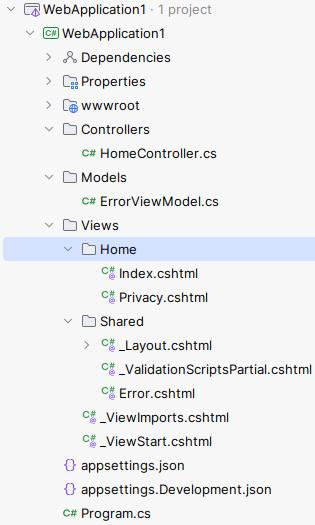
\includegraphics[width=0.2\textwidth]{slike/MVC_project.jpeg}
    \caption{Prikaz MVC u ASP.NET MVC projektu (Izvor: autor)}
    \label{fig:mvc_projekt}
\end{figure}

\subsubsection{Model}
Unutar konteksta ASP.NET MVC projekta, model predstavlja C\# klasu koja sadrži svojstva za spremanje podataka kojima upravljamo. Model je neovisan o korisničkom sučelju ali često će postojati pregled (engl. \textit{View}) koji odgovara za prikaz i upravljanje modelom.
Model također može sadržavati poslovnu logiku za upravljanje podacima, iako to nije učestala praksa i često se ta uloga daje servisima.
\subsubsection{View}
Pregledi (eng. \textit{Views}) se koriste za prikazivanje podataka i korisničku interakciju. ASP.NET MVC koristi Razor stranice, sa ekstenzijom \textit{cshtml}. Razor stranice omogućavaju pisanje C\# koda unutar HTML datoteka koji služi za interaktiranje sa HTML oznakama za generiranje web sadržaja \cite{Smith2022}. Najčešće će svaki pregled imati svoj kontroler koji je odgovoran za rad s pregledima.

\subsubsection{Controllers}
Kontroler u ASP.NET Core MVC arhitekturi služi kao posrednik između modela i prikaza. On obrađuje korisničke zahtjeve, upravlja podacima iz modela, i odlučuje koji će prikaz biti vraćen korisniku. Kontroleri su ključni dio MVC uzorka jer povezuju poslovnu logiku s korisničkim sučeljem.
Kontroler je klasa koja obično nasljeđuje baznu klasu \texttt{Controller} i sadrži metode koje se nazivaju akcije (engl. \textit{actions}). Svaka akcija odgovara određenom korisničkom zahtjevu i vraća rezultat, kao što je prikaz (\textit{ViewResult}), JSON podaci (\textit{JsonResult}), ili redirekcija (\textit{RedirectResult}).
Akcije također možemo opisati kao metode koje se povezivaju kad unesemo određeni URL \cite{Walther2022}.

\subsection{ASP.NET Web API}
ASP.NET Core nam omogućava da kreiramo web API s upotrebom kontrolera koji su usredočeni na resurse i primanje HTTP zahtjeva. Prednost kreiranja zasebnog Web API projekta je da ga može koristiti više različitih vrsta klijenta \cite{ASPNet2023}.
U ASP.NET Core možemo imati dva pristupa kreiranja API-ja:
\begin{itemize}
    \item \textbf{API bazirani na kontrolerima (engl. \textit{controller-based APIs})}: U ovom pristupu, kontroleri (engl. \textit{controllers}) su klase koje nasljeđuju \texttt{ControllerBase} klasu. Ove klase koriste se za definiranje API krajnjih točaka (engl. \textit{endpoints}). Metode unutar kontrolera mapiraju se na određene HTTP zahtjeve (engl. \textit{HTTP requests}, npr. GET, POST) i vraćaju odgovore u obliku JSON-a, XML-a, ili drugih formata.

    \item \textbf{Minimalni API-ji (engl. \textit{minimal APIs})}: Ovaj pristup omogućava definiranje krajnjih točaka pomoću lambda izraza (engl. \textit{lambda expressions}) ili metoda, bez potrebe za punom klasom kontrolera. Minimalni API-ji su dizajnirani za jednostavne i brze implementacije, gdje se fokusira na definiranje krajnjih točaka uz minimalno opterećenje infrastrukture.
\end{itemize}
Za potrebe ovog rada koristit će se API bazirani na kontrolerima zbog bolje organizacije koda u cjeline te zbog jednostavnijeg rukovanja ulaznim podacima pomoću atributa \textit{[FromBody]} i \textit{[FromQuery]} 

\chapter{Izrada Meeting Planner aplikacije}
\section{Uvod u projekt}
Prije izrade projekta trebaju se definirati funckionalnosti projekta. Cilj aplikacije je dohvatiti sve dostupne termine koje korisnik ima u svome Google kalendaru te sinkronizacija u jedan ispis koji će organizatoru sastanka prikazati kada su dostupni svi planirani korisnici i odabrana dvorana u kojoj će se sastanak održati. 
Na bazi toga, definiramo funkcionalnosti.
\begin{itemize}
    \item Prijava korisnika: Korisnik se može prijaviti u sustav koristeći svoje Google podatke.
    \item Prikaz kalendara jednog korisnika (organizator): Korisniku se prikazuje njegov osobni kalendar s pregledom svih zakazanih sastanaka u obliku tablice.
    \item Upis termina u kalendare (kalendar organizatora i kalendar korisnika): Nakon pronalaska slobodnog termina, sustav će omogućiti organizatoru upis sastanka u svoj kalendar kao i njihove kalendare.
    \item Pronalazak slobodnih termina: Sustav pretražuje slobodne termine za sastanak uzimajući u obzir slobodno vrijeme sudionika, odabrane dane za sastanak i dostupne lokacije.
\end{itemize}
Za omogućavanje integracije s Google kalendarom koristiti ćemo Google Calendar API. RESTFul API s kojim se može komunicirati pomoću HTTP poziva.
\section{Dizajn rješenja}

U ovoj sekciji opisujemo dizajn rješenja za aplikaciju \textit{MeetingPlanner}, koja se sastoji od klijentskih {engl. \textit{Frontend}} i poslužiteljskih {engl. \textit{Backend}} komponenti. UML class dijagrami koji prate ovaj opis ilustriraju strukturu ključnih klasa i njihovu međusobnu povezanost.

\subsection{Struktura klijentskog dijela aplikacije}

Na slici \ref{fig:frontend-uml} prikazan je class dijagram za klijentski dio aplikacije \textit{MeetingPlanner} i uključuje sve dijelove \textit{MeetingPlannerFrontend} projekta. Ovaj dio aplikacije uključuje logiku za dohvaćanje slobodnih termina, autentifikaciju korisnika putem Google usluga, te rad s kalendarima korisnika.

\begin{figure}[H]
    \centering
    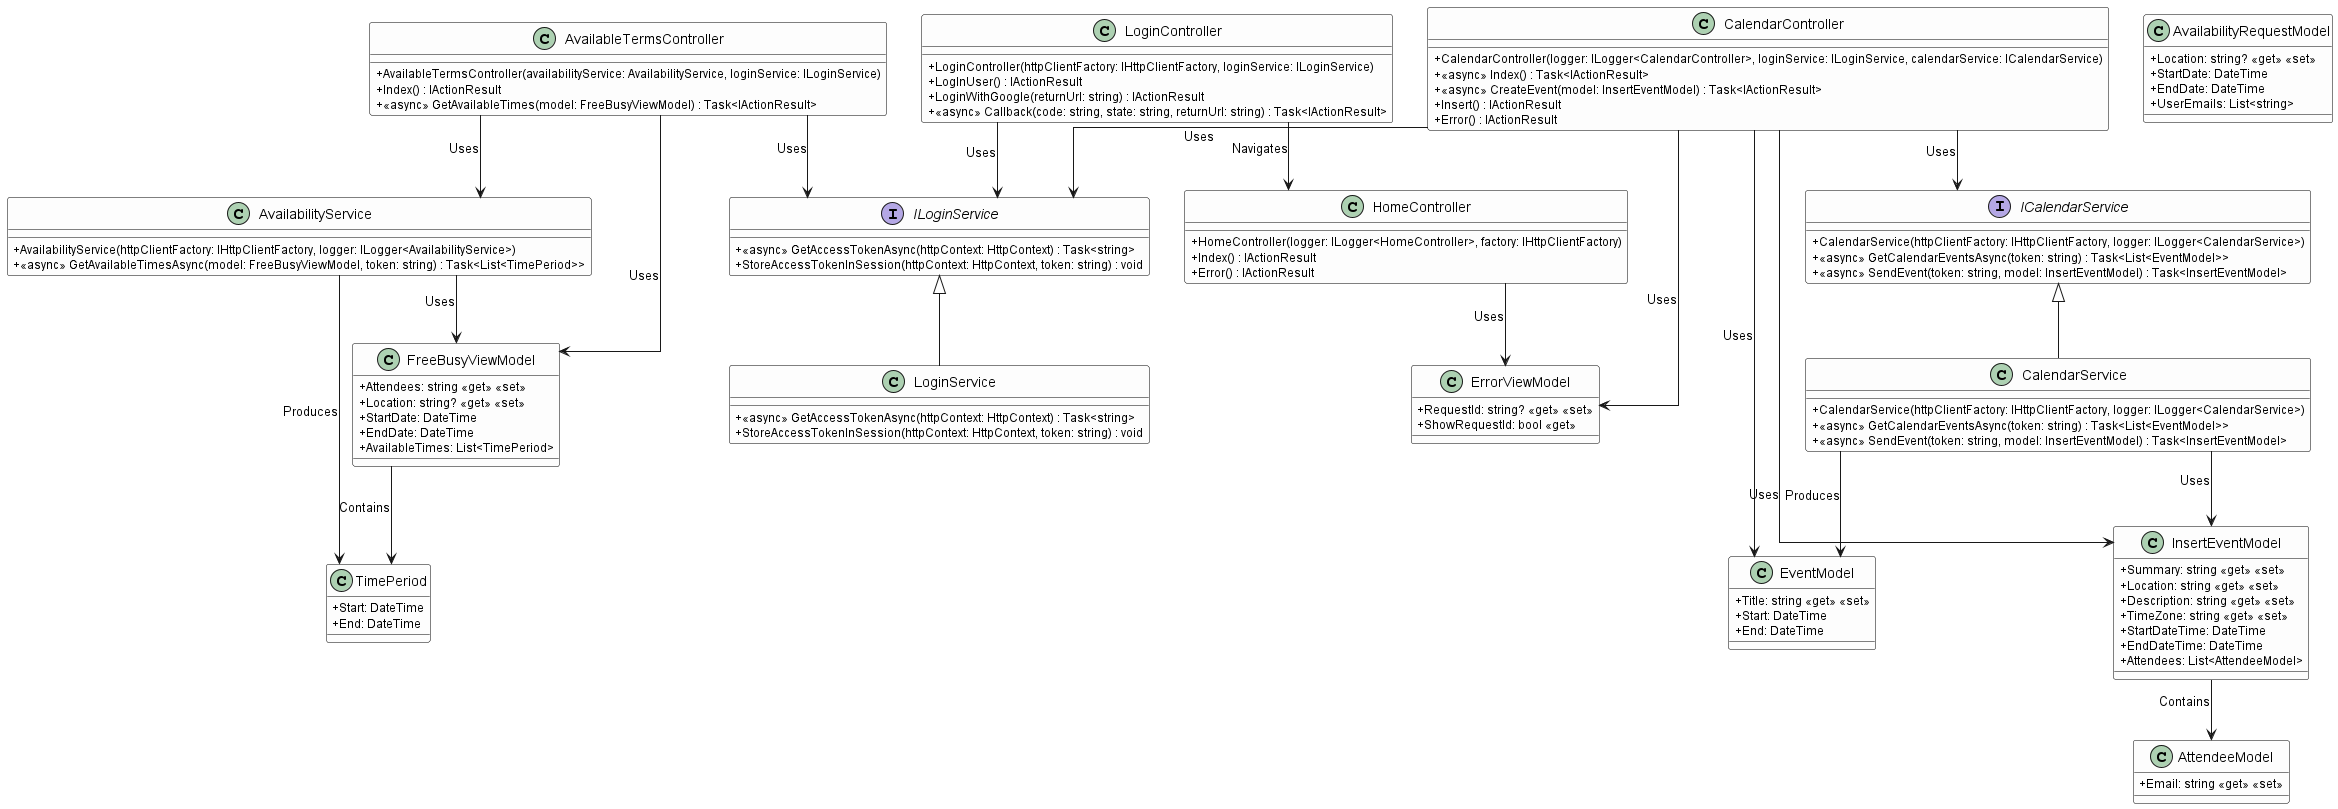
\includegraphics[width=1\textwidth]{slike/MeetingPlannerFrontend_ClassUML.png}
    \caption{Dijagram klasa klijentskog dijela aplikacije}
    \label{fig:frontend-uml}
\end{figure}

Na dijagramu vidimo sljedeće glavne klase i njihove odnose:
\begin{itemize}
    \item \texttt{AvailableTermsController} koristi \texttt{AvailabilityService} kako bi dohvaćao slobodne termine korisnika. Ova klasa je odgovorna za primanje zahtjeva od korisnika i prikaz raspoloživih termina.
    \item \texttt{LoginController} i \texttt{LoginService} rješavaju autentifikaciju korisnika koristeći Google OAuth 2.0. \texttt{LoginService} je odgovoran za dobivanje pristupnog tokena i njegovo spremanje u sesiju.
    \item \texttt{CalendarController} i \texttt{CalendarService} omogućuju interakciju s Google kalendarom korisnika, uključujući kreiranje i dohvaćanje događaja.
    \item Modeli kao što su \texttt{FreeBusyViewModel}, \texttt{AvailabilityRequestModel}, i \texttt{InsertEventModel} definiraju strukturu podataka koja se koristi za prikaz informacija o zauzetim terminima, slanje zahtjeva i kreiranje događaja.
\end{itemize}

\subsection{Struktura poslužiteljskog dijela}

Poslužiteljsko rješenje je prikazano na slici \ref{fig:backend-uml}, koja uključuje ključno poslovno logiku za rad s Google Calendar API-em i korisničkim autentifikacijskim tokovima.

\begin{figure}[H]
    \centering
    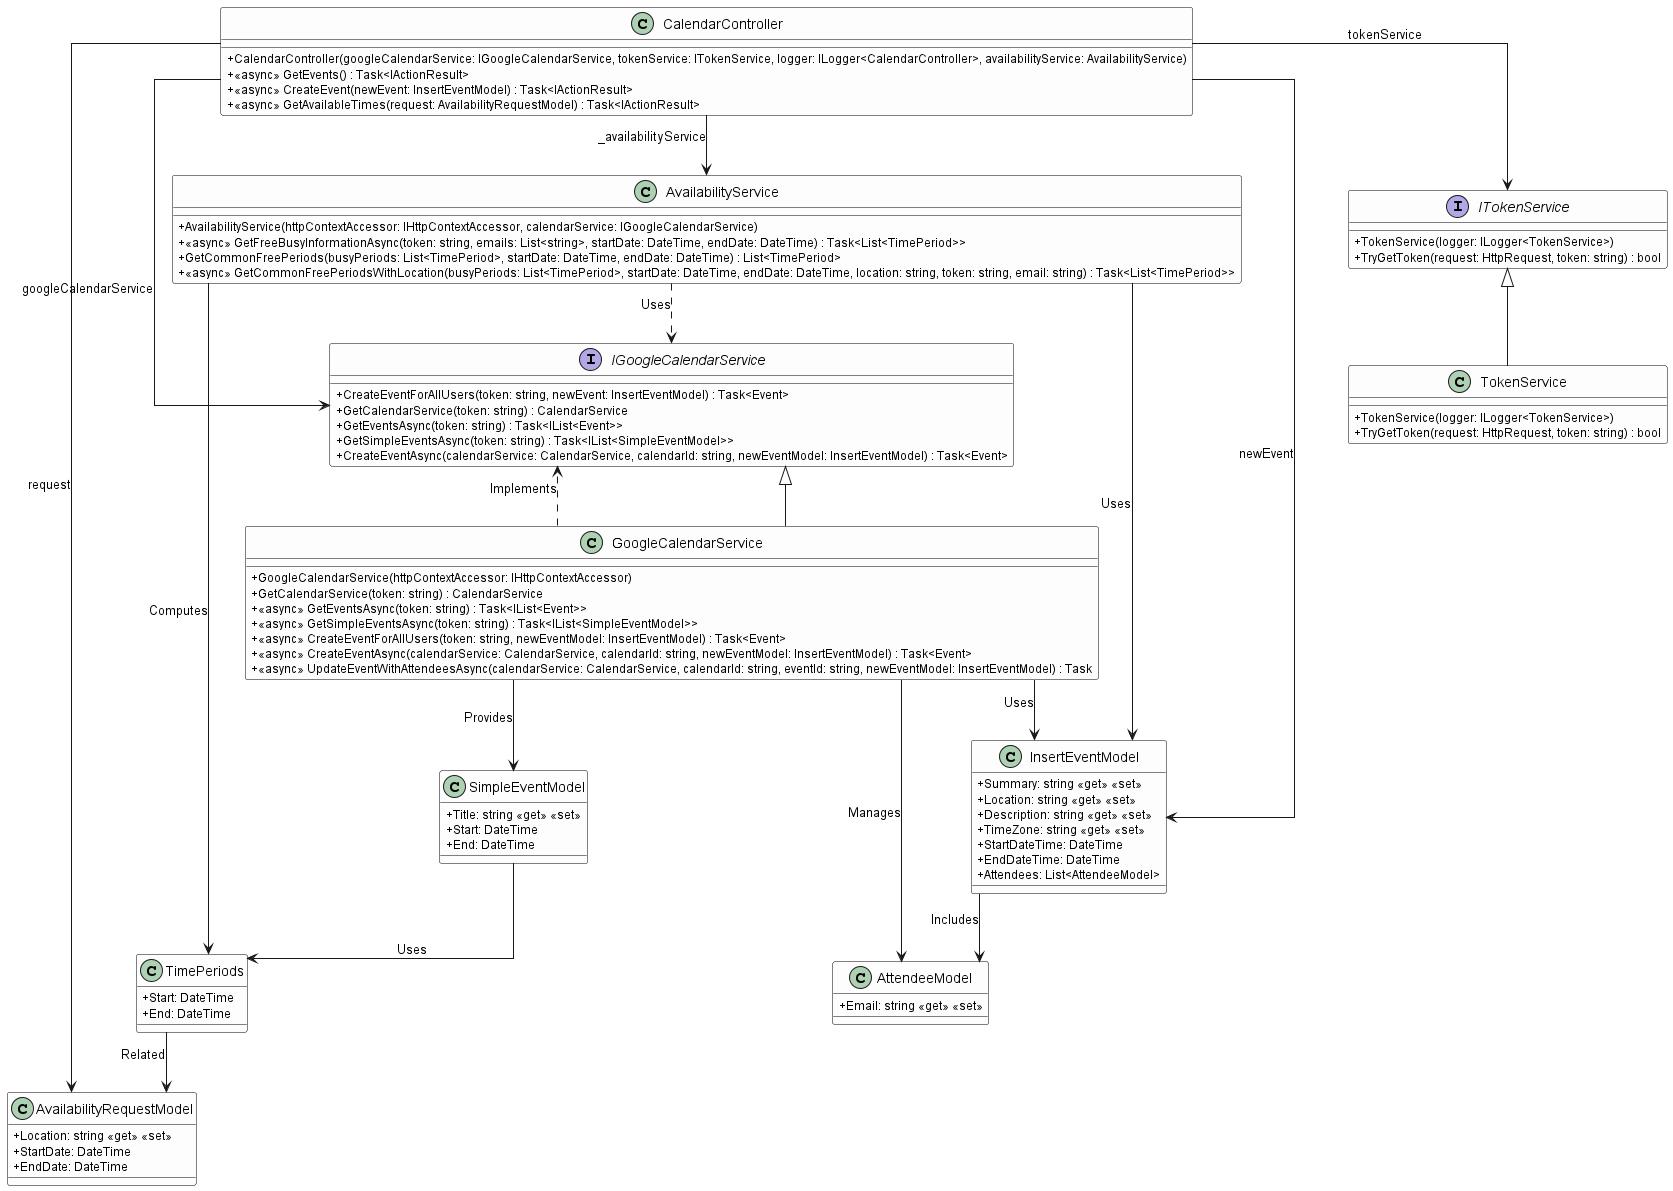
\includegraphics[width=0.8\textwidth]{slike/MeetingPlannerAPI_ClassUML.png}
    \caption{Class dijagram poslužiteljske komponente}
    \label{fig:backend-uml}
\end{figure}

Na dijagramu vidimo sljedeće klase i njihove funkcionalnosti:
\begin{itemize}
    \item \texttt{CalendarController} je glavni kontroler koji koristi \texttt{AvailabilityService} za dohvaćanje slobodnih termina iz Google kalendara, kao i za kreiranje novih događaja.
    \item \texttt{AvailabilityService} koristi \texttt{IGoogleCalendarService} kako bi obavljao složene operacije nad kalendarima korisnika, poput dohvaćanja zauzetih termina i kombiniranja slobodnih perioda.
    \item \texttt{GoogleCalendarService} implementira stvarnu komunikaciju s Google Calendar API-jem, obavljajući pozive za dohvaćanje i ažuriranje događaja.
    \item Modeli kao što su \texttt{InsertEventModel}, \texttt{SimpleEventModel}, i \texttt{AvailabilityRequestModel} definiraju strukturu podataka potrebnu za komunikaciju s API-em, kao i za spremanje informacija o događajima.
\end{itemize}


\section{Google Workspace}
Google Workspace nam omogućava platformu za integraciju Google Workspace alata kao što su Maps, Calendar ili Sheets. Za ovaj projekt su nam potrebni Google Workspace APIs da integriramo kalendar s našim rješenjem.
Da možemo koristiti te servise moramo prvo stvoriti projekt u Google Cloud konzoli te omogućiti Google Calendar API za naš projekt.
\begin{figure}[H]
    \centering
    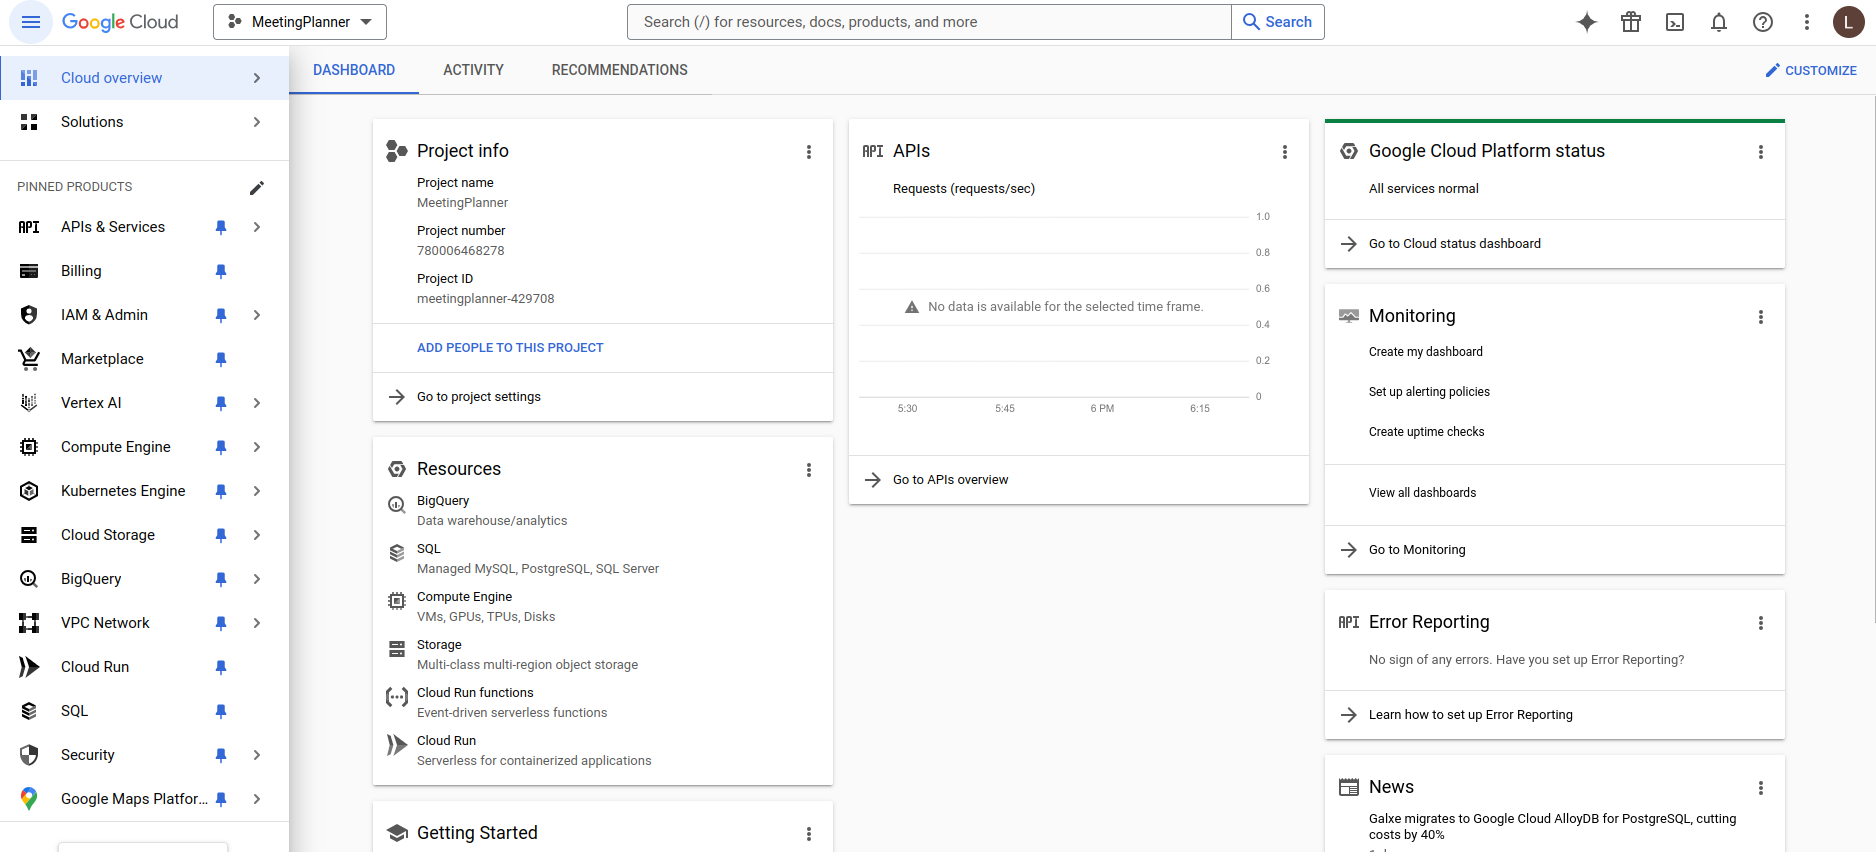
\includegraphics[width=0.9\textwidth]{slike/google_console.png}
    \caption{Google Cloud console (Izvor: autor)}
    \label{fig:google_console}
\end{figure}
Potrebno je imati aktivni Google email račun, te se prijaviti u \textit{Google Cloud Console}. Kreiranje projekta je dosta intuitivno, najbitniji korak je omogućiti google calendar API
\begin{figure}[H]
    \centering
    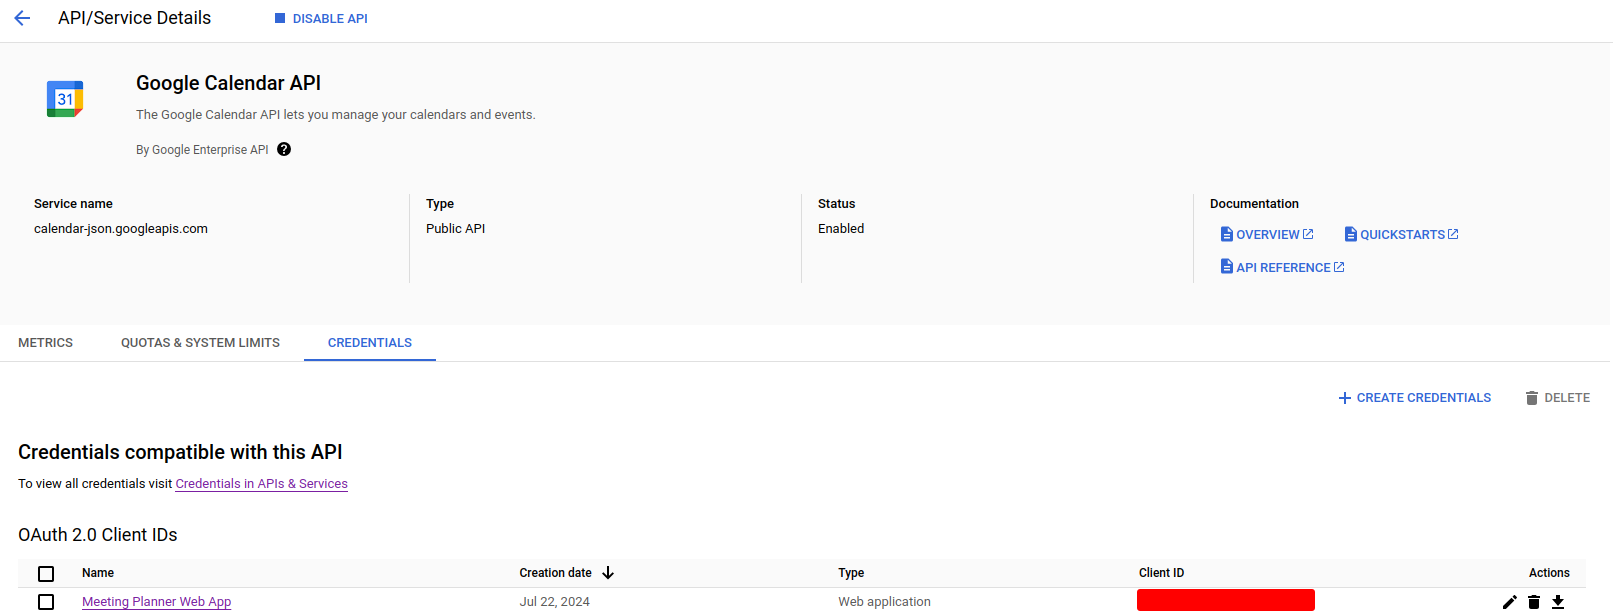
\includegraphics[width=0.8\textwidth]{slike/enabledGoogleCalendarAPI.png}
    \caption{Omogućavanje Google Calendar API (Izvor: autor)}
    \label{fig:enabledGoogleCalendarAPI}
\end{figure}

Generira se tajna klijenta koji nam je potreban da naša aplikacija može slati zahtjeve Google API-ju.
\begin{figure}[H]
    \centering
    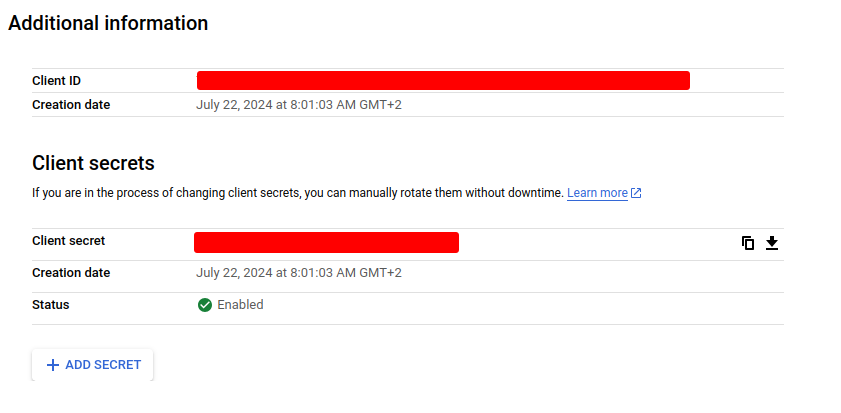
\includegraphics[width=0.8\textwidth]{slike/additionalINfo.png}
    \caption{Informacije o projektu MeetingPlanner (Izvor: autor)}
    \label{fig:additionalINfo}
\end{figure}

Za proces razvoja aplikacije potrebno je dodati \textit{TestUsers} koji se mogu prijavljivati u našu aplikaciju
\begin{figure}[H]
    \centering
    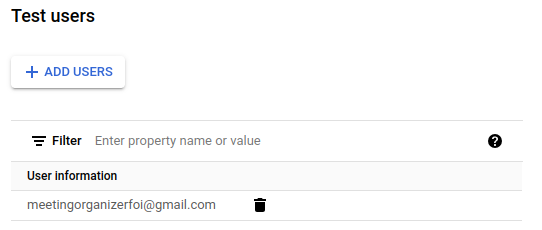
\includegraphics[width=0.8\textwidth]{slike/TestUSers.png}
    \caption{Informacije o projektu MeetingPlanner (Izvor: autor)}
    \label{fig:TestUsers}
\end{figure}

\section{Stvaranje projekta}
Za stvaranje projekta prvo je potrebno stvoriti prazno rješenje (engl. \textit{Solution}), te kreirati zasebni WEB API i MVC projekt.
\begin{figure}[H]
    \centering
    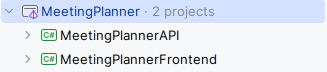
\includegraphics[width=0.6\textwidth]{slike/struktura.png}
    \caption{Rješenje MeetingPlanner (Izvor: autor)}
    \label{fig:struktura}

\end{figure}
Za dodatnu konfiguraciju potrebno je preuzeti json datoteku koja sadrži podatke koji našoj aplikaciji omogućuju pozivanje google servisa. 
\begin{itemize}
    \item GoogleId (Identifikator klijenta): jedinstveni identifikator dodijeljen aplikaciji od strane Googlea. Identificira vašu aplikaciju na Googleovim poslužiteljima prilikom slanja zahtjeva, kao što su autentifikacija korisnika ili pristup API-jima.
    \item GoogleSecret (Tajni ključ): povjerljivi ključ povezan s vašom Google aplikacijom. Koristi se zajedno s GoogleId za autentifikaciju vaše aplikacije prema Googleu.
\end{itemize}
\newpage
\section{Autentifikacija}
Kako bi korisnik aplikacije mogao pristupiti vanjskim uslugama on mora biti prijavljen, korisnik će se prijavljivati putem svojeg Google računa koristeći OAuth 2.0 protokol. Prvo je potrebno konfigurati autentifikaciju projekta u \textit{Program.cs} datoteci.
\begin{figure}[H]
    \centering
    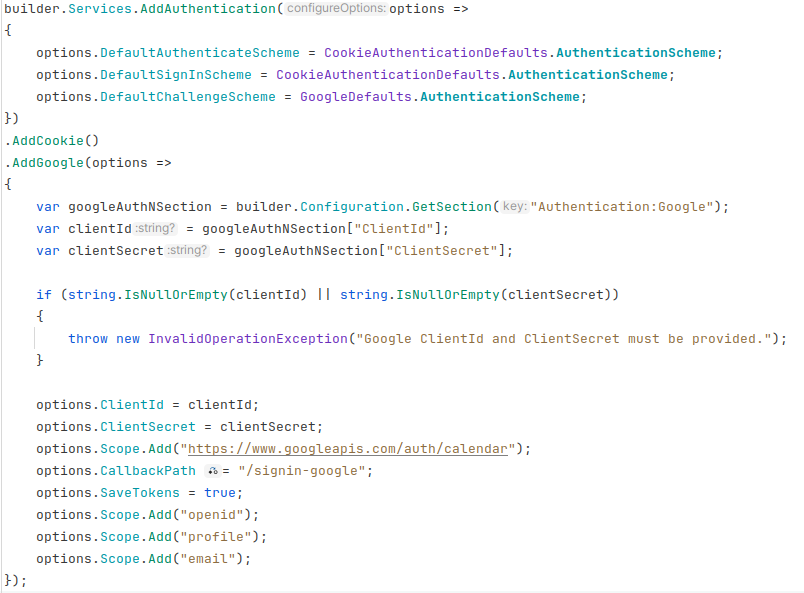
\includegraphics[width=0.7\textwidth]{slike/auth.png}
    \caption{Postavljanje autentifikacije (Izvor: autor)}
    \label{fig:autentifikacija_programcs}
\end{figure} Kod konfigurira autentifikaciju postavljanjem kolačića za prijavu i koristeći Google za autentifikaciju korisnika, uključujući konfiguraciju za Google kalendar, pohranu OAuth tokena, i određivanje putanje za povratak korisnika nakon prijave.
Kada je postavljena konfiguracija kreiramo login stranicu, s obzirom da koristimo Google autentifikaciju kreiramo element koji poziva akciju \textit{LoginWithGoogle}.
\begin{figure}[H]
    \centering
    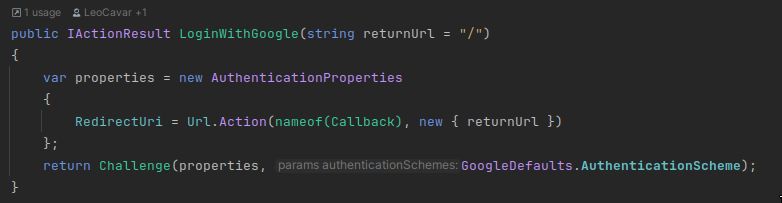
\includegraphics[width=0.9\textwidth]{slike/loginwithgoogle.png}
    \caption{Metoda LoginWithGoogle (Izvor: autor)}
    \label{fig:LoginWithGoogle}

\end{figure}
\newpage
Metoda \textit{LoginWithGoogle} inicijalizira objekt \textit{AuthenticationProperties} s postavkom \textit{RedirectUri} koja određuje putanju na metodu \textit{Callback} nakon prijave putem Googlea. Metoda \texttt{Challenge} pokreće izazov za autentifikaciju koristeći Google kao pružatelja, preusmjeravajući korisnika na Google za prijavu ako nije već prijavljen. Nakon uspješne prijave, korisnik će biti vraćen na metodu \texttt{Callback} gdje se token sprema u sesiju što nam omogućava autorizirane API pozive.
\begin{figure}[H]
    \centering
    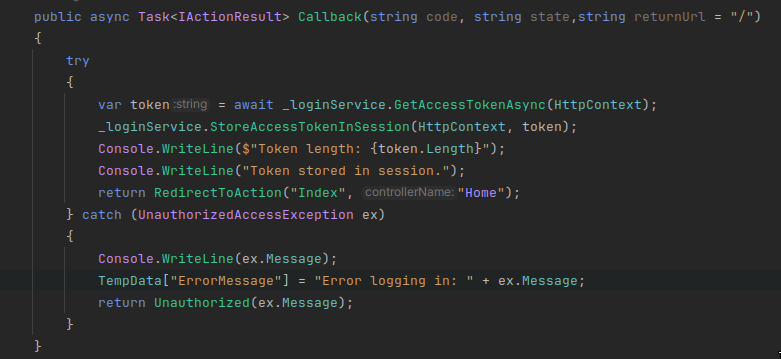
\includegraphics[width=0.9\textwidth]{slike/callbackFunction.png}
    \caption{Metoda Callback (Izvor: autor)}
    \label{fig:Callback}

\end{figure}
Za spremanje podataka u sesiju definira se metoda \textit{StoreAccessTokenInSession}. Metoda se nalazi u zasebnom login servisu unutar kojega se također nalazi metoda za dohvaćanje tokena za kasniju upotrebu \textit{GetAccessTokenAsync}.
\begin{figure}[H]
    \centering
    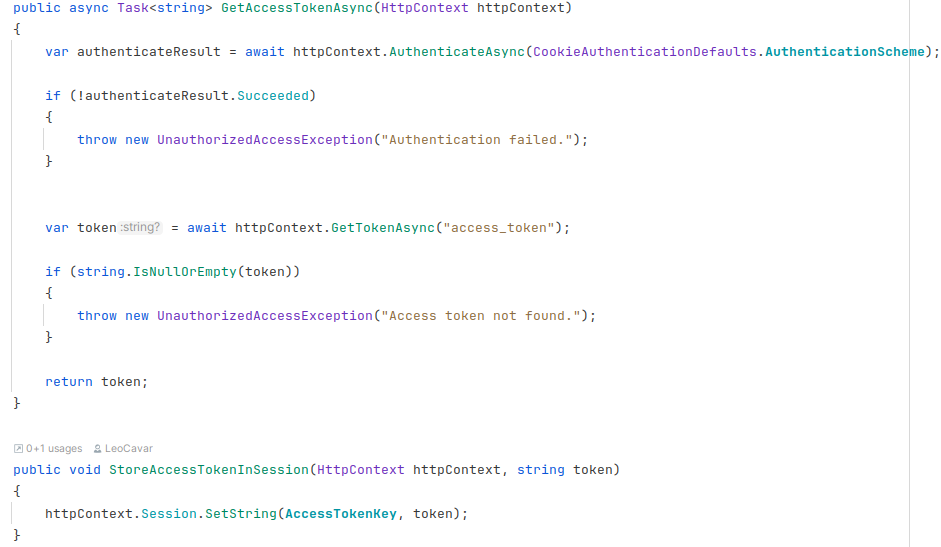
\includegraphics[width=0.9\textwidth]{slike/storeToken.png}
    \caption{Login servis (Izvor: autor)}
    \label{fig:StoreAccessTokenInSession}

\end{figure}






\section{Prikaz događaja}
Za prikaz događaja implementiramo zaseban pregled {eng. \textit{View}}. Koristiti će se mogućnost razor stranica da se upisuje C\# kod i definirat će se jednostavna provjera varijable \textit{isLoggedIn}. 
\begin{figure}[H]
    \centering
    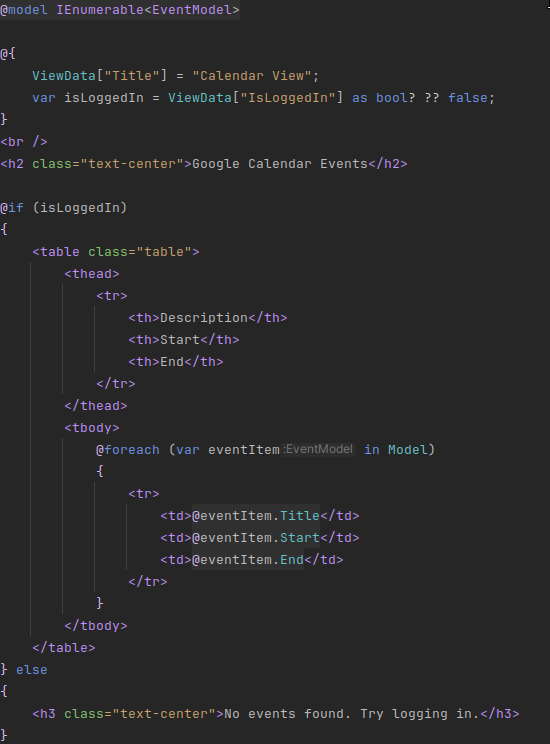
\includegraphics[width=0.6\textwidth]{slike/calendarView.png}
    \caption{Pregled kalendara (Izvor: autor)}
    \label{fig:calendarView}

\end{figure}
Definira se klasa \textit{EventModel} koja sadrži naslov, vrijeme početka i vrijeme kraja događaja. Klasa služi za mapiranje događaja koje dobivamo pozivom API-ju u korisniku lako čitljiv oblik. 
Nakon definiranja ispisa događaja, potrebno je implementirati logiku unutar kontrolera i servisa. Kontroler nam služi za obradu zahtjeva dok se sva poslovna logika i interakcija s podacima izvršava u servisu {\textit{CalendarService}}.
\begin{figure}[H]
    \centering
    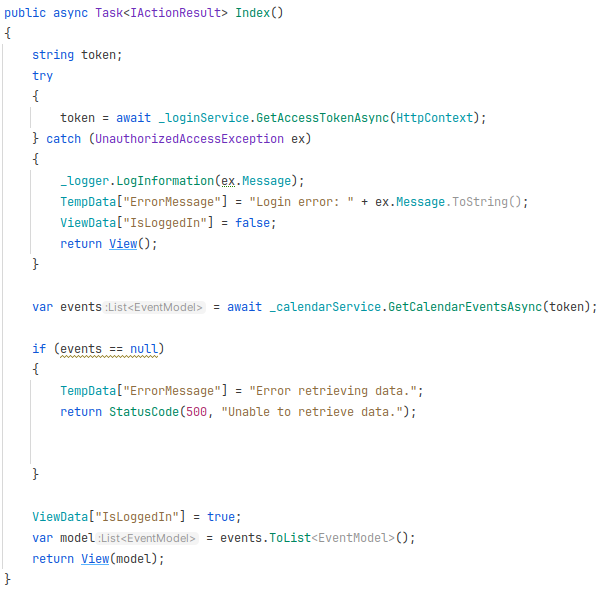
\includegraphics[width=0.9\textwidth]{slike/cControllerIndex.png}
    \caption{Pregled kalendara kontroler (Izvor: autor)}
    \label{fig:ctrl}

\end{figure}
Kontroler dohvaća token pomoću funkcije \textit{GetAccessTokenAsync} te poziva metodu \textit{GetCalendarEventsAsync} koristeći token da pošalje poziv API-ju te upravlja greškama koristeći try/catch metode. 
Unutar \textit{CalendarService} metoda \textit{GetCalendarEventsAsync} stvara klijent pod imenom "API", to je klijent koji sadrži putanju na poslužitelja koji sadrži API krajnja točke.
Zahtjevu se dodaje token u \textit{AuthenticationHeaderValue} da se mogu dohvatiti podaci i šalje se zahtjev na definiranu krajnja točku "\textit{calendar/events}".
\begin{figure}[H]
    \centering
    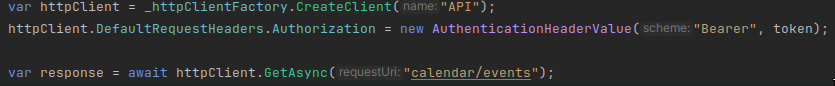
\includegraphics[width=0.9\textwidth]{slike/calendarRequest.png}
    \caption{Slanje zahtjeva na API krajnja točku za dohvaćanje kalendara (Izvor: autor)}
    \label{fig:calendarRequest}

\end{figure}
Odgovor se mapira iz JSON stringa u .NET objekt, u ovom kontekstu se pretvara u \textit{EventModel}.
\begin{figure}[H]
    \centering
    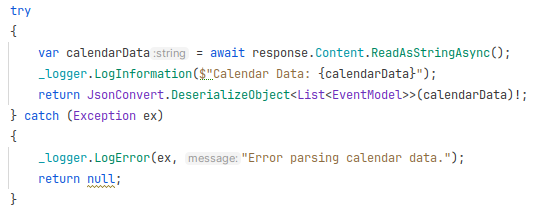
\includegraphics[width=0.9\textwidth]{slike/calendarReturn.png}
    \caption{Metoda za upravljanjem povratnog JSON teksta (Izvor: autor)}
    \label{fig:calendarReturnList}

\end{figure}
Ovo je sva potrebna logika za klijentski dio sustava. Potrebno je implementirati poslužiteljski dio.
Poslužiteljski dio se implementira tako što se definira \textit{ApiController} ruta koja se pozvala u metodi \textit{GetCalendarEventsAsync}. 
Prvobitno se izvršava validacija tokena te se dohvaćaju događaji pomoću metode \textit{GetSimpleEventsAsync} i provjerava se uspješnost operacije.
\begin{figure}[H]
    \centering
    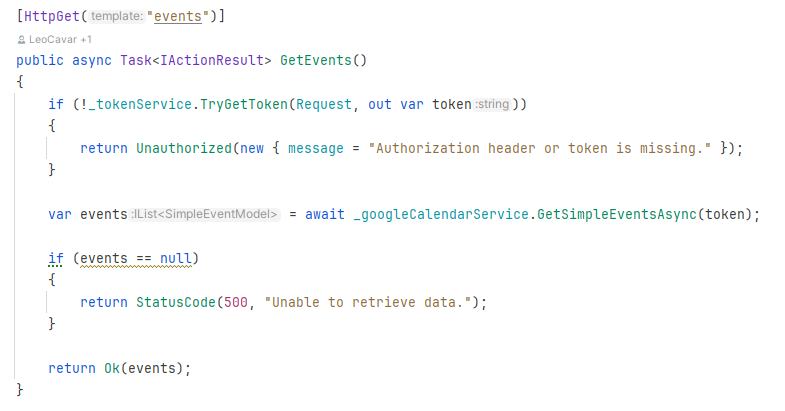
\includegraphics[width=0.9\textwidth]{slike/GetCalendarEventsEndpoint.png}
    \caption{Kalendar "events" krajnja točka (Izvor: autor)}
    \label{fig:GetCalendarEventsEndpoint}

\end{figure}
Metoda za dohvaćanje se sastoji od dva dijela, prvi dio je stvaranje instance \textit{CalendarService}. Ovaj servis je od GoogleAPI-ja te nam omogućava manipulaciju podacima autoriziranog korisnika unutar google kalendara.
\begin{figure}[H]
    \centering
    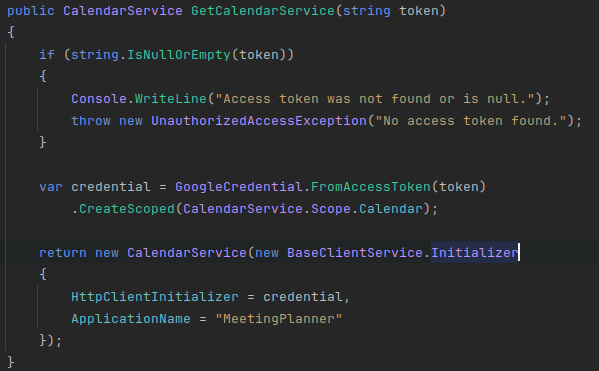
\includegraphics[width=0.9\textwidth]{slike/GetCalendarService.png}
    \caption{Metoda za dohvaćanje instance Google kalendar servisa (Izvor: autor)}
    \label{fig:GetCalendarService}

\end{figure}
Drugi dio procesa je dohvaćanje \textit{Events.List} resursa i mapiranje u obliku \textit{SimpleEventModel}.
\begin{figure}[H]
    \centering
    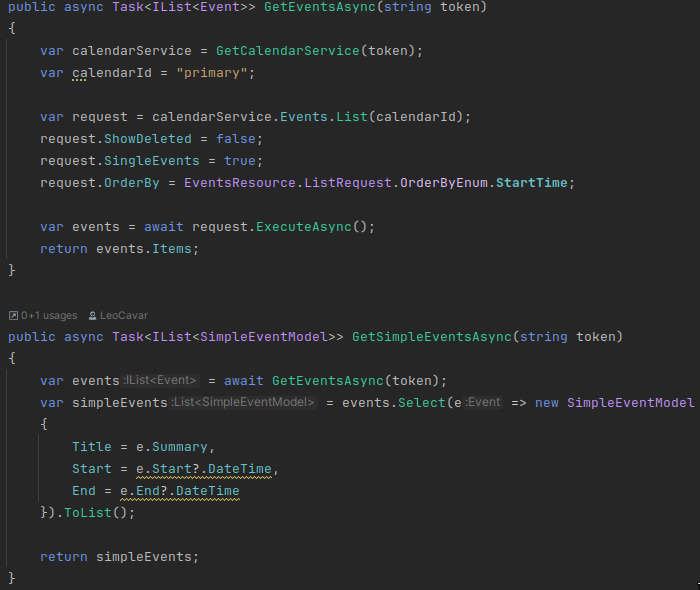
\includegraphics[width=0.8\textwidth]{slike/GetSimpleEventAsync.png}
    \caption{Metoda GetSimpleEventAsync (Izvor: autor)}
    \label{fig:GetSimpleEventAsync}
\end{figure}
Nakon implementacije metode naša funkcionalnost je potpuna, te se kalendar vraća u obliku tablice prijavljenom korisniku.
\begin{figure}[H]
    \centering
    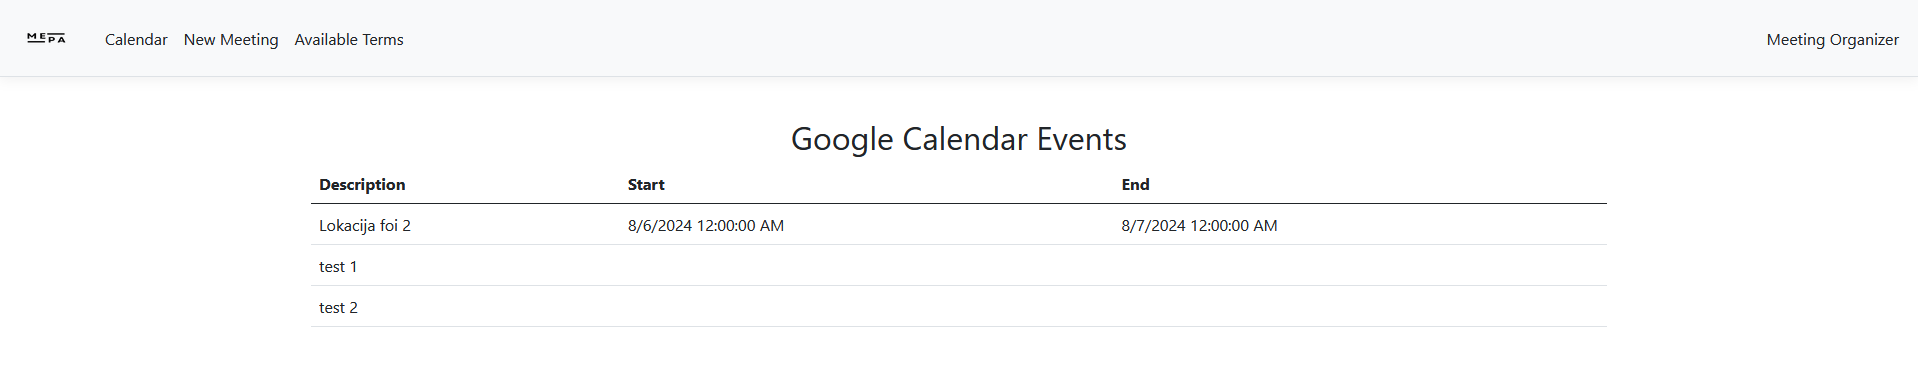
\includegraphics[width=0.8\textwidth]{slike/calendarEvents.png}
    \caption{Prikaz kalendara na web stranici (Izvor: autor)}
    \label{fig:CalendarViewImg}
\end{figure}
\section{Protok podataka}

Protok podataka u ovoj aplikaciji je jasno definiran za sve funkcionalnosti koje će se implementirati dalje u ovome radu s malim razlikama ovisno o funkcionalnosti ali uzorak će ostati isti.
\begin{itemize}
    \item \textbf{Klijentov zahtjev}: Korisnik putem web aplikacije odabire funkcionalnost koju želi koristiti putem korisničkoj sučelja te se šalje odgovarajući zahtjev
    \item \textbf{Obrada zahtjeva na poslužitelju}: Poslužiteljski kontroler prima zahtjev i prosljeđuje ga odgovarajućem servisu.
    \item \textbf{Autentifikacija i autorizacija}: Prilikom dohvaćanja podataka iz Google Calendar API-ja, aplikacija koristi OAuth 2.0 autentifikaciju. Token za pristup provjerava se i koristi za autentifikaciju zahtjeva prema Googleovim uslugama.
    \item \textbf{Odgovor poslužitelja}: Nakon obrade podataka, poslužitelj šalje odgovor klijentu. Ovaj odgovor uključuje popis slobodnih termina za sve korisnike u traženom vremenskom periodu, koji se klijentu vraćaju u JSON formatu ili potvrdu o izmjeni i unosu podataka.
    \item \textbf{Prikaz rezultata klijentu}: Klijentska aplikacija prima JSON odgovor i prikazuje slobodne termine korisniku u vizualno preglednom formatu, omogućujući mu da jednostavno vidi kada su svi korisnici dostupni ili se prikazuje odgovarajuća greška ovisno o odgovoru.
\end{itemize}
\begin{figure}[H]
    \centering
    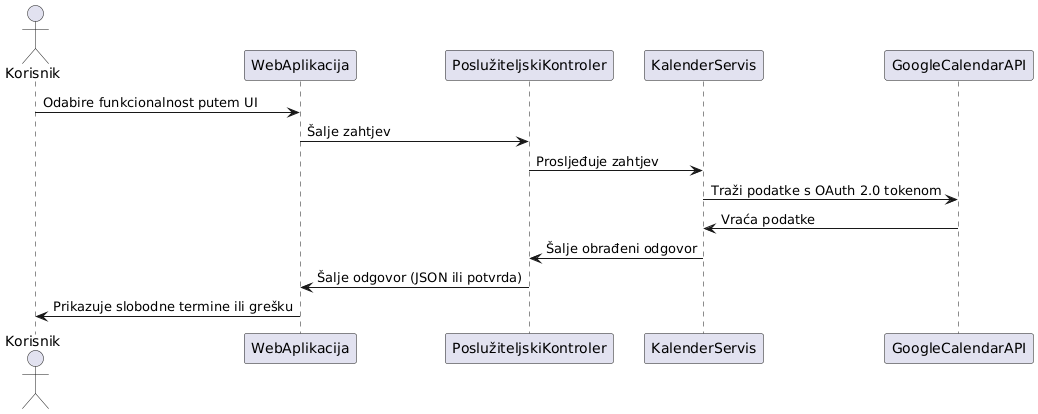
\includegraphics[width=0.8\textwidth]{slike/protokPodataka.png}
    \caption{Prikaz slijeda protoka podataka  (Izvor: autor)}
    \label{fig:protokPodataka}
\end{figure}
\section{Pronalazak slobodnih termina}
Kako Google Calendar API ne omogućuje izravno dohvaćanje slobodnih termina, postupak pronalaska slobodnih perioda obuhvaća sljedeće korake:
\begin{itemize}
    \item Dohvat kalendara svih dolaznika (engl. \textit{Attendees})
    \item Filtriranje kalendara po lokaciji
    \item Identificiranje zauzetih termina unutar zadanog vremenskog raspona
    \item Kombiniranje svih zauzetih termina kako bi se pronašli zajednički slobodni periodi
    \item Oduzimanje zauzetih termina od cijelog vremenskog raspona kako bi se identificirali slobodni termini
\end{itemize}

Korisničko sučelje uključuje obrazac koji šalje zahtjev na \textit{calendar/get-available-times} nakon unosa podataka. Odgovor se prikazuje u tablici sa slobodnim periodima.

\begin{figure}[H]
    \centering
    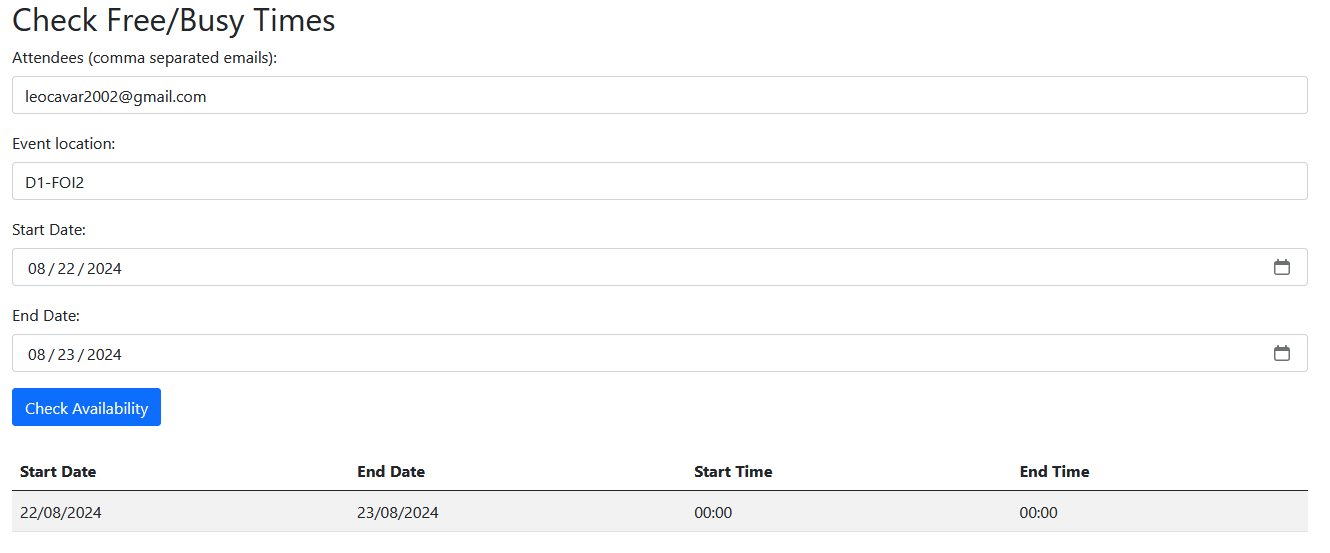
\includegraphics[width=0.7\textwidth]{slike/timesAvaileble.png}
    \caption{Web sučelje za prikaz dostupnih termina (Izvor: autor)}
    \label{fig:UserInterfaceAvailible}
\end{figure}

Funkcija \textit{GetAvailableTimesAsync} vraća popis objekata \textit{TimePeriod} koji sadrži vrijeme početka i kraja slobodnog perioda. Zahtjev uključuje token u headeru, a u tijelu se nalaze vremenski period, lokacija i email adrese korisnika. Funkcija šalje POST zahtjev na \textit{get-available-times} krajnju točku, koji zatim prosljeđuje zahtjev metodi \textit{GetCommonFreePeriodsWithLocation} nakon validacije tokena i zahtjeva.
Unutar akcije \textit{GetAvailableTimes} na koju se šalje zahtjev dohvaćaju se prvo svi termini kada su korisnici zauzeti.
\begin{figure}[H]
    \centering
    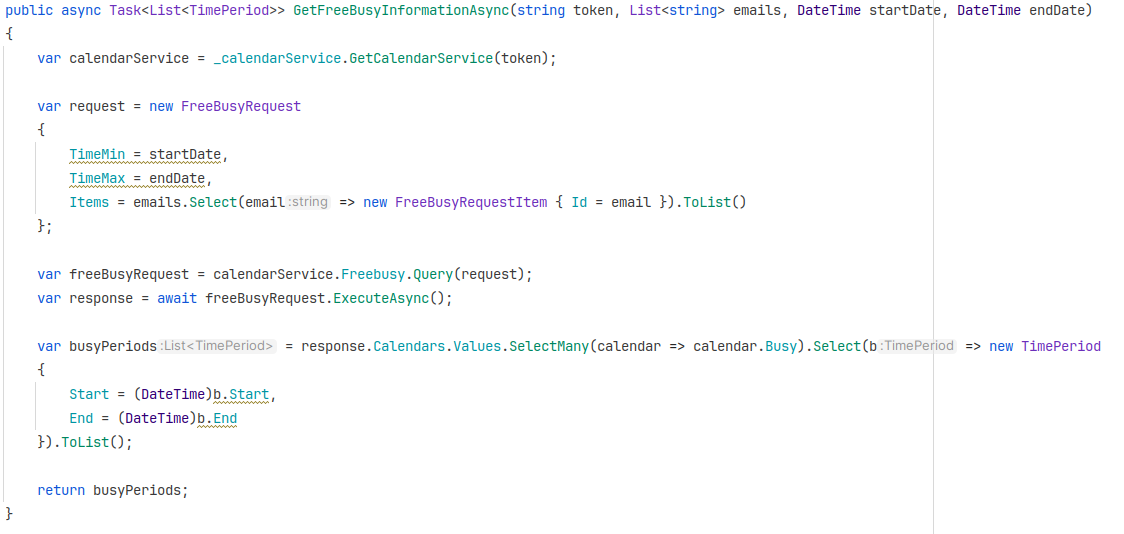
\includegraphics[width=0.7\textwidth]{slike/getfreebuisy.png}
    \caption{Metoda \textit{GetFreeBusyInformationAsync} (Izvor: autor)}
    \label{fig:GetFreeBusyInformationAsync}
\end{figure}
Nakon dohvaćanja zauzetih termina za sve korisnike, potrebno je preuzeti termine kada je dvorana zauzeta.
\begin{figure}[H]
    \centering
    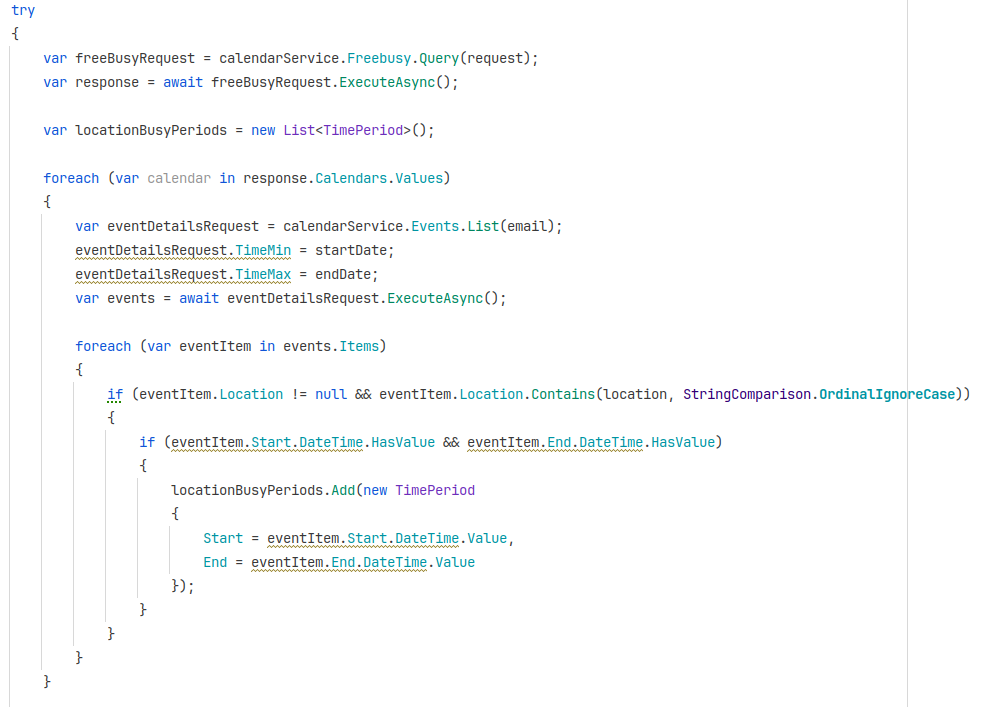
\includegraphics[width=0.7\textwidth]{slike/GetBuisyLocation.png}
    \caption{Dohvaćanje zauzetih termina odabrane lokacije (Izvor: autor)}
    \label{fig:GetBuisyLocation}
\end{figure}
Nakon preuzimanja termina lokacije imamo sve potrebne podatke, prvo je potrebno spojiti zauzete periode korisnika s zauzetim terminima dvorane, metoda \textit{Concat} omogućava da spojimo periode u jednu varijablu \textit{combinedBusyPeriods}.
Nakon spajanja u jednu varijablu, moramo pretvoriti popis zauzetih termina u popis slobodnih termina. Implementira se metoda \textit{GetCommonFreePeriods} i kao povratna vrijednost klijentu se vraćaju svi slobodni periodi.
\begin{figure}[H]
    \centering
    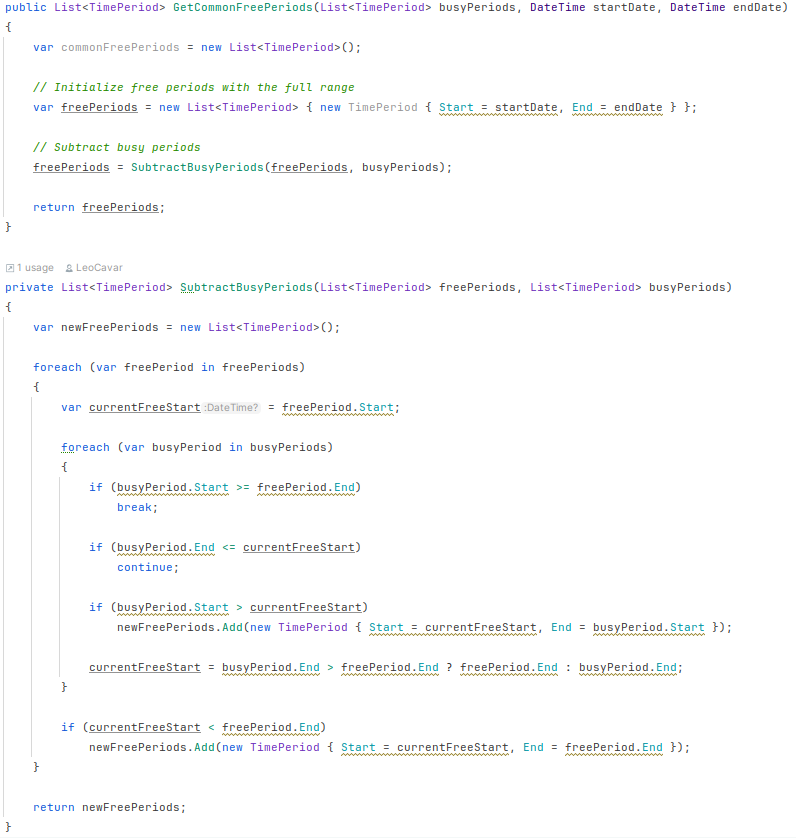
\includegraphics[width=0.8\textwidth]{slike/FreePeriods.png}
    \caption{Metode za pretvaranje zauzetih termina u slobodne (Izvor: autor)}
    \label{fig:FreePeriods}
\end{figure}
Metode \textit{GetCommonFreePeriods} i \textit{SubtractBusyPeriods} instanciraju popis \textit{TimePeriod} unutar odabranog vremenskog raspona te pomoću metode \textit{SubtractBusyPeriods} se od slobodnih vremena oduzimaju zauzeta vremena, stvarajući popis u kojemu se nalaze svi slobodni termini korisnika.
\begin{figure}[H]
    \centering
    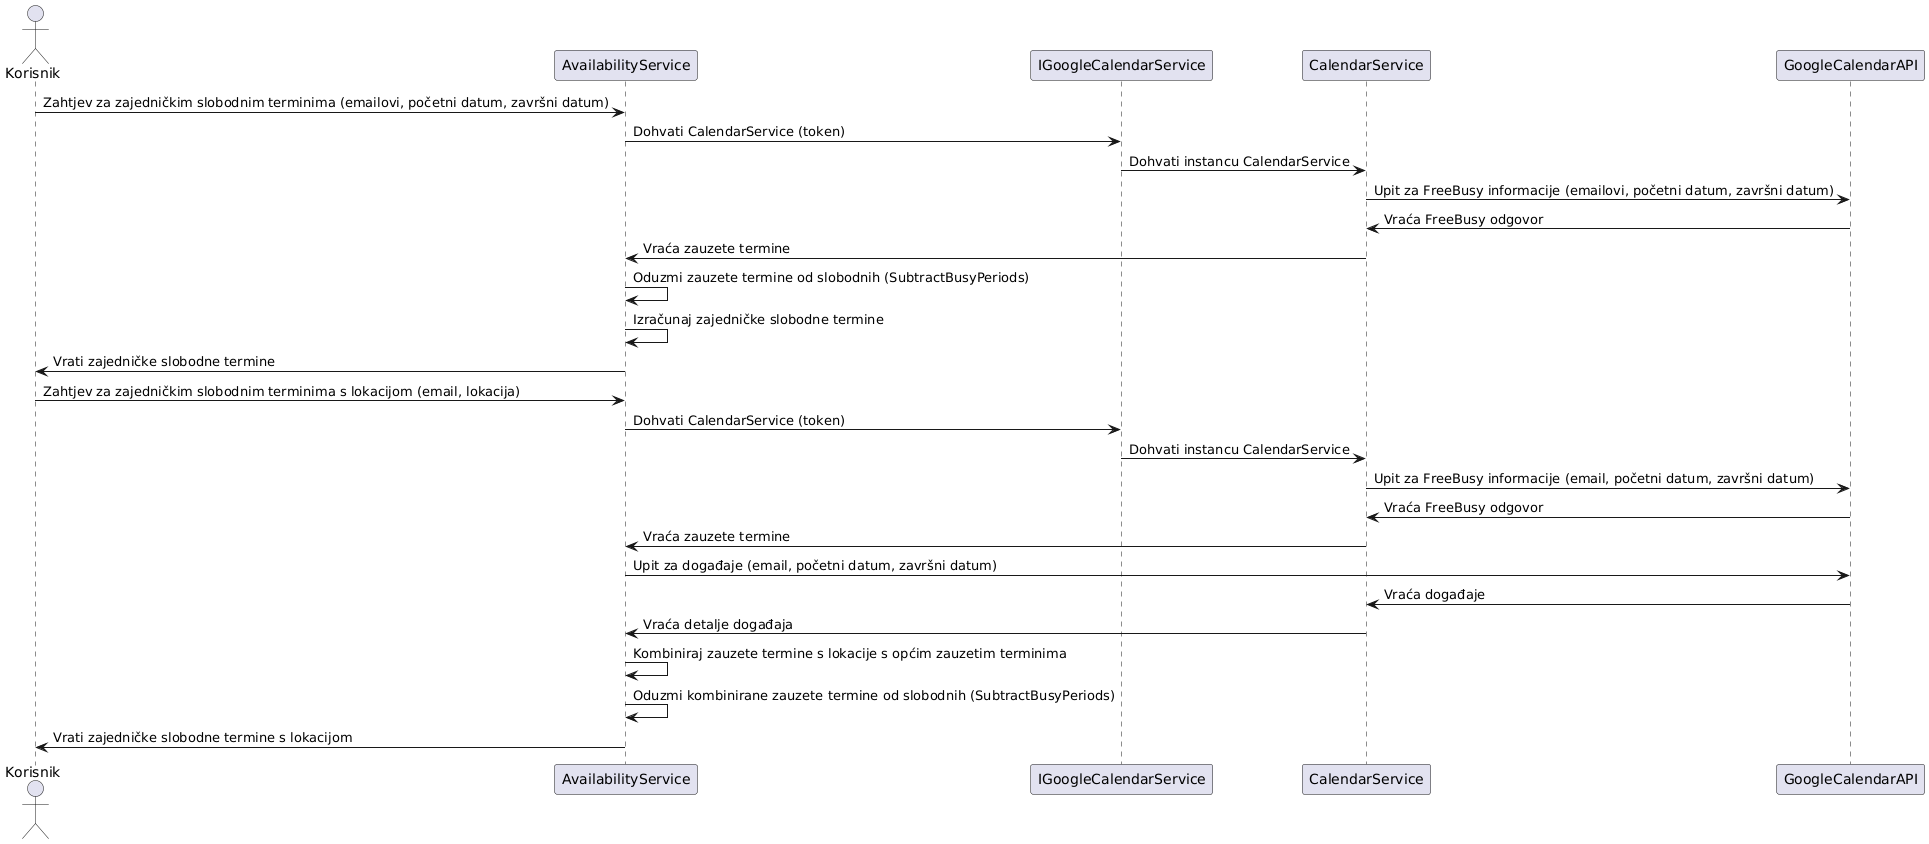
\includegraphics[width=0.9\textwidth]{slike/dijagramSlijedaFreePeriods.png}
    \caption{Dijagram slijeda pronalaska slobodnog termina (Izvor: autor)}
    \label{fig:dijagramSlijedaFreePeriods}
\end{figure}
\section{Unos sastanka}
Kao završni dio aplikacije potrebno je omogućiti korisniku da unosi aktivnosti u kalendare korisnika. Prvo je potrebno kreirati sučelje za unos, korisnik može unositi opis, lokaciju sastanka, opis , vremenski period aktivnosti, vremensku zonu i goste sastanka.
\begin{figure}[H]
    \centering
    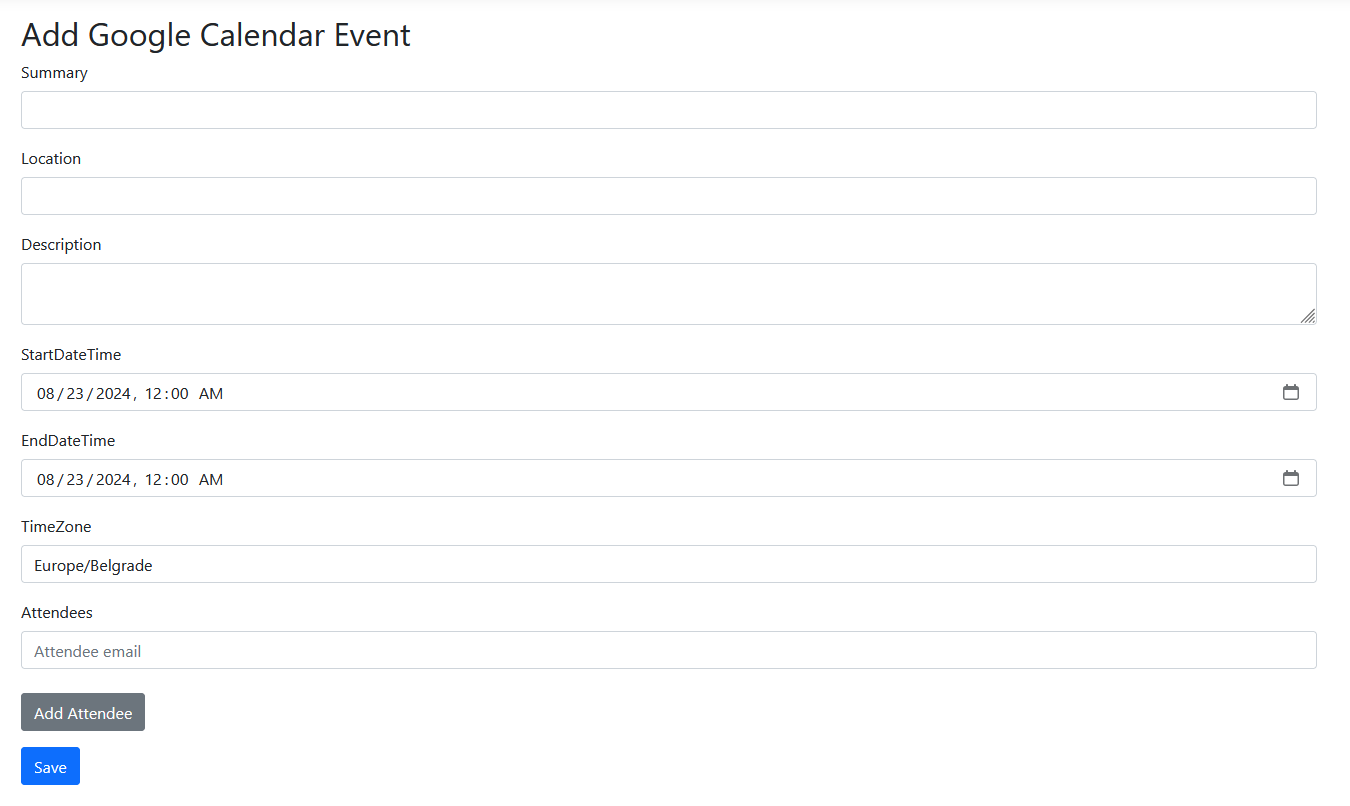
\includegraphics[width=0.8\textwidth]{slike/insertMeeting.png}
    \caption{Sučelje za unos sastanka (Izvor: autor)}
    \label{fig:InsertMeeting}
\end{figure}
Potrebno je poslati POST zahtjev s svim parametrima, uneseni podaci se mapiraju u klasu \textit{InsertEventModel} te se šalju na \textit{calendar/events} krajnju točku. Stvara se novi \textit{Event} objekt u kalendaru organizatora, te se na taj događaj dodaju članovi.
\begin{figure}[H]
    \centering
    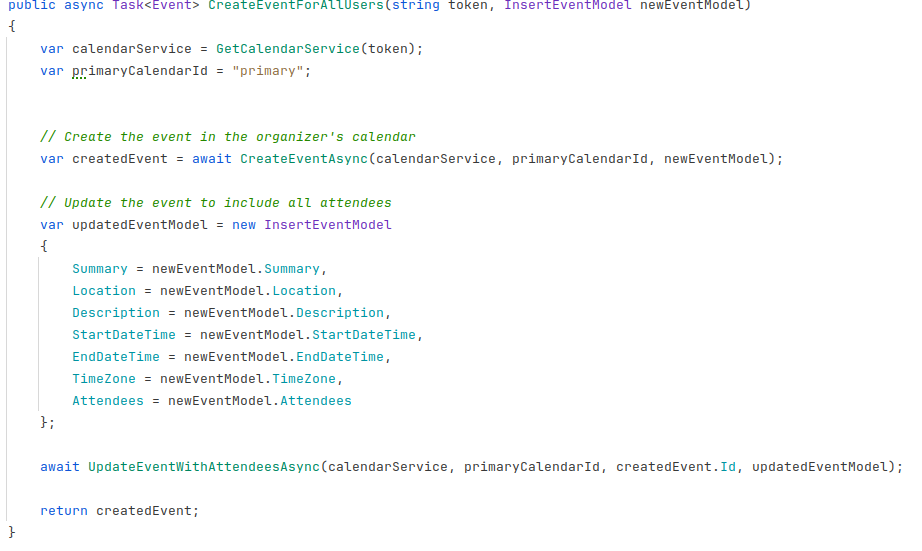
\includegraphics[width=0.8\textwidth]{slike/createEventForAllUsers.png}
    \caption{Implementacija unosa događaja u kalendare korisnika (Izvor: autor)}
    \label{fig:createEventForAllUsers}
\end{figure}

\section{Demonstracija korištenja aplikacije}
Kada korisnik dođe na stranicu prvo se prezentira poruka pozdrava i navigacija.
\begin{figure}[H]
    \centering
    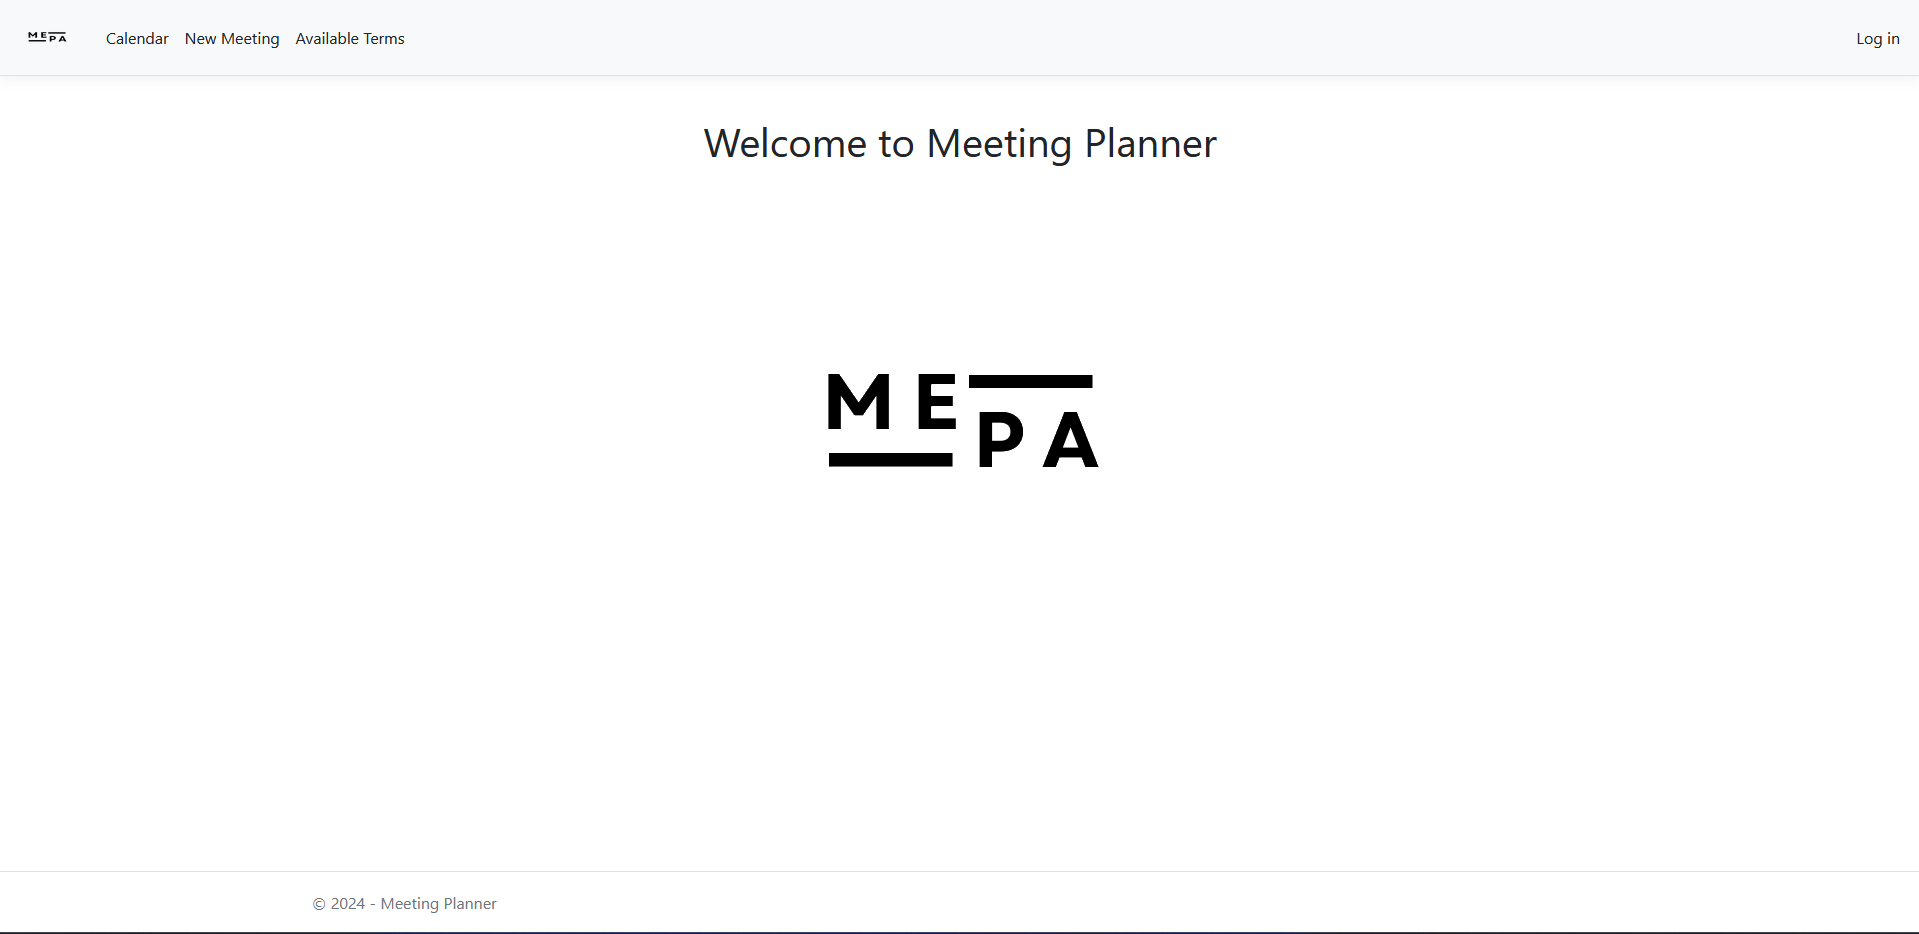
\includegraphics[width=0.8\textwidth]{slike/appUsage1.png}
    \caption{Početna stranica (Izvor: autor)}
    \label{fig:startPageUI}
\end{figure}
Prije nego što može koristiti funkcionalnosti aplikacije korisnik se mora prijaviti sa Google računom.
\begin{figure}[H]
    \centering
    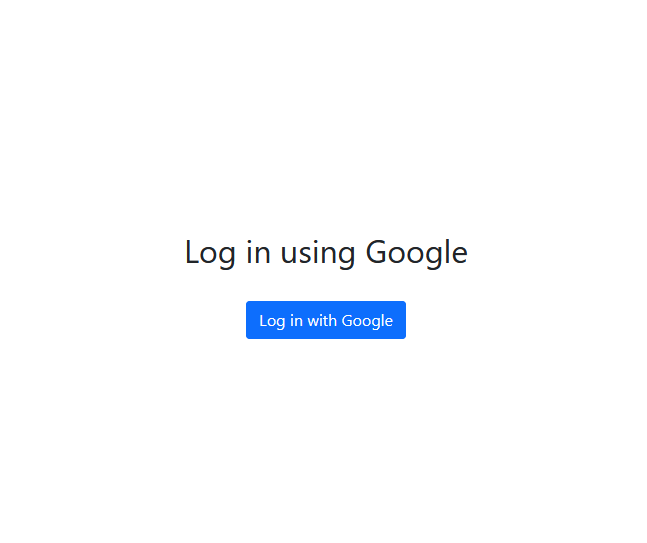
\includegraphics[width=0.8\textwidth]{slike/appUsage2.png}
    \caption{Login stranica (Izvor: autor)}
    \label{fig:loginUI}
\end{figure}
Kada ode na stranicu \textit{Calendar} korisniku se prikazuju njegovi događaji u kalendaru
\begin{figure}[H]
    \centering
    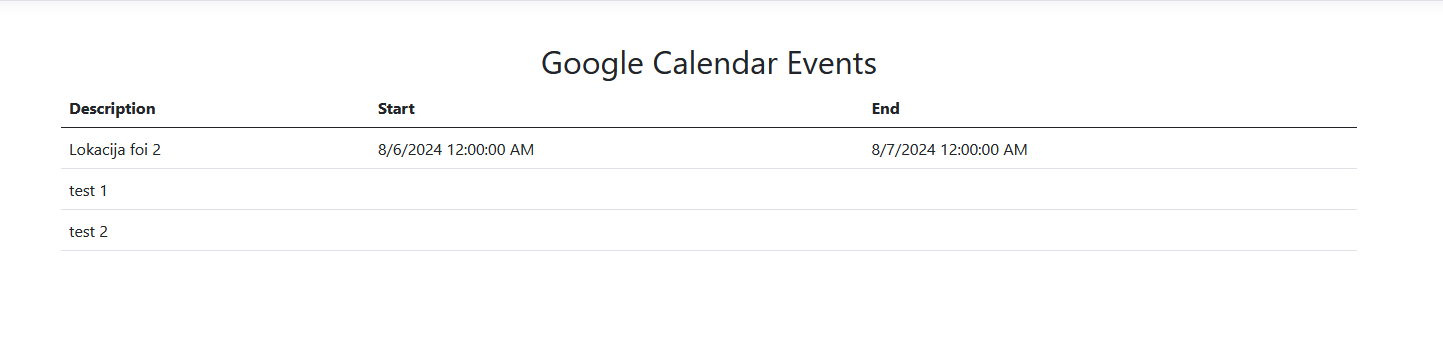
\includegraphics[width=0.8\textwidth]{slike/appUsage3.png}
    \caption{Kalendar prijavljenog korisnika (Izvor: autor)}
    \label{fig:userCalendarUI}
\end{figure}
Korisnik uzima u obzir svoje termine te provjerava kalendare korisnika. Unosi podatke o korisniku za kojeg se provjerava termin te se automatski ulogirani korisnik dodaje u provjeru i dobiva povratnu informaciju o slobodnim terminima.
\begin{figure}[H]
    \centering
    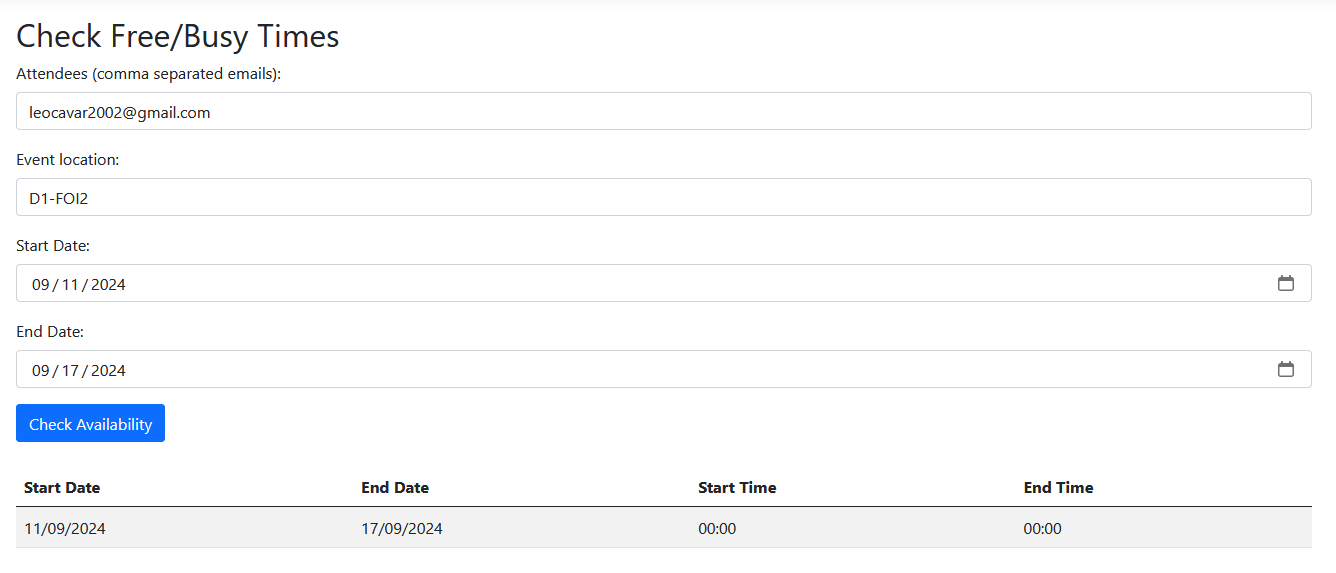
\includegraphics[width=0.8\textwidth]{slike/appUsage4.png}
    \caption{Provjera dostupnosti korisnika (Izvor: autor)}
    \label{fig:createEventForAllUserss}
\end{figure}
Uvidom u kalendar gostiju sastanka korisnik ima opciju dodati novi sastanak u kalendare korisnika. Korisnik unosi odgovarajuće podatke te unosi sastanak u kalendare svih korisnika.
\begin{figure}[H]
    \centering
    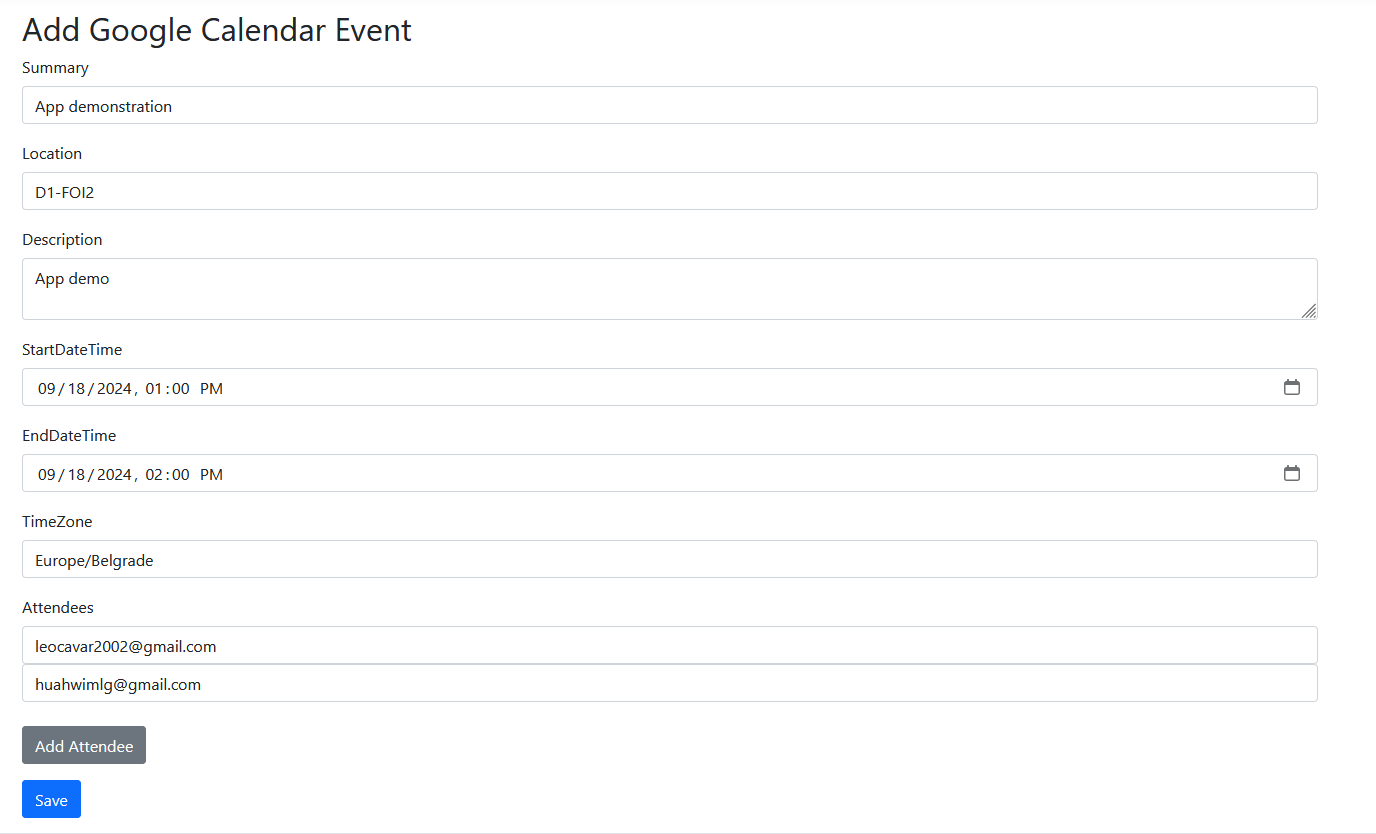
\includegraphics[width=0.8\textwidth]{slike/appUsage5.png}
    \caption{Korisničko sučelje za unos sastanka (Izvor: autor)}
    \label{fig:InputMEetingUI}
\end{figure}
Korisniku se daje odgovarajuća poruka ako je sastanak uspješno unesen.
\begin{figure}[H]
    \centering
    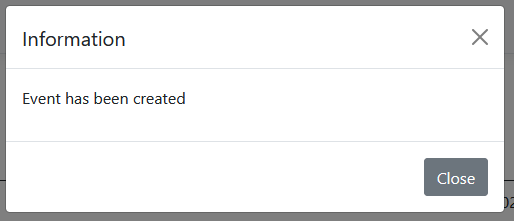
\includegraphics[width=0.8\textwidth]{slike/appUsage6.png}
    \caption{Potvrda o unosu sastanka (Izvor: autor)}
    \label{fig:meetingconfirmPOpUp}
\end{figure}
Kada gosti sastanka otvore svoj google kalendar vide sastanak koji smo unjeli u njegov kalendar te je taj događaj prisutan i u kalendaru organizatora.
\begin{figure}[H]
    \centering
    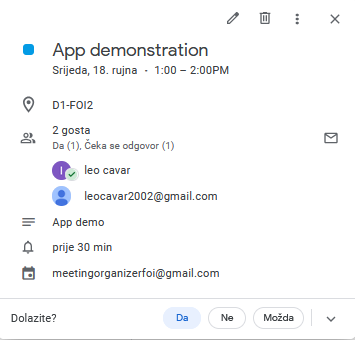
\includegraphics[width=0.8\textwidth]{slike/appUsage7.png}
    \caption{Stvoreni događaj u kalendaru korisnika (Izvor: autor)}
    \label{fig:GCUserUI}
\end{figure}

\chapter{Zaključak}

Zaključno, ovaj rad pruža sveobuhvatan prikaz procesa izrade aplikacije za planiranje sastanaka koristeći Google Calendar API, razvijene u ASP.NET Core tehnologiji. Detaljno objašnjenje koje je uključeno u rad omogućava bolje razumijevanje glavnih funkcionalnosti aplikacije, uključujući autentifikaciju korisnika putem OAuth 2.0 protokola, dohvaćanje i manipulaciju događajima iz Google kalendara, te njihovo prikazivanje i upravljanje unutar aplikacije.

Rad se detaljno osvrće na tehničke aspekte implementacije, s posebnim naglaskom na uporabu RESTful API-ja i MVC arhitekture. RESTful API omogućava učinkovit prijenos podataka između klijenta i poslužitelja, čime se osigurava brza i pouzdana komunikacija koja je ključna za funkcioniranje aplikacije. MVC (Model-View-Controller) arhitektura doprinosi organizaciji koda i odvojenosti odgovornosti, što poboljšava održivost i proširivost aplikacije. Razdvajanjem poslovne logike, prikaza i kontrole korisničkog sučelja, MVC arhitektura omogućava lakše upravljanje i nadogradnju aplikacije.

Korištenje Google Workspace API-ja omogućilo je integraciju vanjskih servisa u aplikaciju, čime je omogućena sinkronizacija i interakcija s Google kalendarima. Ova integracija značajno povećava funkcionalnost aplikacije, omogućujući korisnicima pristup informacijama o svojim i tuđim kalendarima u realnom vremenu. Time se značajno olakšava planiranje sastanaka, jer korisnici mogu provjeriti dostupnost svih sudionika i odabrati optimalno vrijeme za održavanje sastanaka.

Osim tehničkog aspekta, rad također naglašava kako se napredne tehnike web razvoja mogu primijeniti za rješavanje konkretnih poslovnih izazova u kontekstu organizacije sastanaka. Razvijena aplikacija ne samo da poboljšava korisničko iskustvo kroz intuitivno sučelje, već i doprinosi većoj efikasnosti u organizaciji sastanaka. Time se smanjuje vrijeme potrebno za pronalaženje zajedničkih slobodnih termina među sudionicima i povećava produktivnost u poslovnim procesima.

Ovaj rad pokazuje kako moderna tehnologija i integracija s vanjskim servisima mogu unaprijediti poslovne procese i organizaciju. Razvijena aplikacija prikazuje pristupačnost i potencijal Google servisa u razvoju samostalnih aplikacija, pružajući korisnicima moćne alate za optimizaciju svojih dnevnih aktivnosti i sastanaka. Izvorni kod i kompletan projekt dostupni su na \href{https://github.com/LeoCavar/MeetingPlanner}{GitHub repozitoriju}.

\printbibliography[title=Popis literature]
\addcontentsline{toc}{chapter}{Popis literature}

\listoffigures
\addcontentsline{toc}{chapter}{Popis slika}


\end{document}
